\documentclass{article}
\usepackage{listings}
\usepackage[T1]{fontenc}
\usepackage{algorithm}
\usepackage{algorithmic}
\usepackage{amsfonts}
\usepackage{tikz}
\usepackage{systeme}
\usepackage{tcolorbox}

% Language setting
% Replace `english' with e.g. `spanish' to change the document language
\usepackage[polish]{babel}

% Set page size and margins
% Replace `letterpaper' with `a4paper' for UK/EU standard size
\usepackage[letterpaper,top=2cm,bottom=2cm,left=3cm,right=3cm,marginparwidth=1.75cm]{geometry}

% Useful packages
\usepackage{amsmath}
\usepackage{inconsolata}
\usepackage{graphicx}
\graphicspath{ {.} }
\usepackage[colorlinks=true, allcolors=blue]{hyperref}
\usepackage{xcolor}
\lstset { %
    language=C++,
    backgroundcolor=\color{black!5}, % set backgroundcolor
    basicstyle=\footnotesize,% basic font setting
}

\title{Algorytm znajdowania sumy podzbioru}
\author{Łukasz Wasilewski}

\begin{document}
\maketitle

\begin{abstract}
Problem istnienia podzbioru o sumie $t$ zawierającego się w $n$-elementowym (multi)zbiorze $S \subset \mathbb{N}$, 
jest jednym z klasycznych problemów algorytmicznych. Problem w ogólności jest problemem $NP$-zupełnym ~\cite{agarwal2011encrypting}
jednak jeżeli $t$ jest względnie małe i dysponujemy pamięcią $\Omega(t)$ istnieją algorytmy działające 
w czasie wielomianowym od długości wejścia, z czego najbardziej znanym jest działający w czasie $O(nt)$ 
algorytm oparty na programowaniu dynamicznym.

Celem niniejszej pracy jest dokumentacja implementacji
algorytmu opracowanego przez Ce Jin i Hongxun Wu w pracy ~\cite{jin2018simple}. Algorytm ten jest niedeterministyczny,
jednak dla dużych danych prawdopodobieństwo błędu jest niewielkie. Złożoność czasowa prezentowanego
algorytmu to $O((t+n)\log^2(t))$, zaś pamięciowa $O(n+t)$.

\end{abstract}

\section{Wstęp}
Problem sprawdzenia czy z $n-$elementowego multizbioru $S$ liczb naturalnych jesteśmy w stanie wybrać 
podzbiór, którego suma elementów jest równa zadanej liczbie $t$ jest jednym z klasycznych problemów 
algorytmicznych. Będziemy go w dalszej części nazywać \textbf{problem sumy podzbioru}. 

Ma on zastosowanie w licznych praktycznych zagadnieniach na przykład kryptografii
~\cite{agarwal2011encrypting}, analizie finansowej 
~\cite{biesner2022solving}, czy zagadnieniach kombinatorycznych, jako specyficzny
wariant problemu plecakowego (Problem plecakowy dotyczy możliwości wybrania ze zbioru przedmiotów, z których każdy ma 
określoną wagę i wartość, podzbioru mającego maksymalną sumaryczną wartość i jednocześnie, którego 
sumaryczna waga nie przekracza pewnej liczby $t$. Problem sumy podzbiorów odpowiada sytuacji, 
gdy wartości przedmiotów są wprost proporcjonalne do ich wagi). 

Klasyczna wersja problemu, gdzie $t$ jest duże (gdy nie dysponujemy $O(t)$ pamięci) jest problemem 
$NP$-zupełnym ~\cite{sasamoto2001statistical}. Najprostszy algorytm rozwiązujący ten problem polega na rozważeniu po kolei wszystkich 
możliwych podzbiorów. Złożoność tego algorytmu to $O(n2^n)$. Nieco szybszym algorytmem jest algorytm Horowitza
i Sahaniego ~\cite{horowitz1974computing} który działa w $O(2^{\frac{n}{2}}n/2)$, jednak w przeciwieństwie do algorytmu naiwnego wymagającego
$O(n)$ pamięci algorytm ten wymaga $O(2^{\frac{n}{2}})$. Algorytm Schroeppela i Shamira ~\cite{schroeppel1981t} wymaga takiego samego
czasu jak algorytm Horowitza i Sahaniego, jednak potrzebuje $O(2^{\frac{n}{4}})$ pamięci. Probabilistyczny 
algorytm Howgrave-Grahama i Jouxa ~\cite{howgrave2010new} pozwolił przyspieszyć rozwiązanie problemu do $O(2^{0.337n})$
zużywając $O(2^{0.256})$ pamięci. Dalsze jego ulepszenia pozwoliły osiągnąć złożoność czasową równą 
$O(2^{0.291n})$ ~\cite{becker2011improved}.

Znacznie mniej czasu wymagają instancje problemu sumy podzbiorów, gdzie $t$ jest względnie małe i dysponujemy
$O(t)$ pamięci. Oparty o programowanie dynamiczne klasyczny algorytm wymaga $O(nt)$ czasu i $O(n+t)$ pamięci.
Używam go do sprawdzenia poprawności implementacji algorytmu Ce Jin i Hongxun Wu. Najszybszym znanym algorytmem deterministycznym
dla problemu sumy podzbiorów z małym $t$ jest algorytm Konstantinos Koiliaris i Chao Xu ~\cite{bach1997comments}. 

Algorytm, który prezentuję w niniejszej pracy został opracowany przez Ce Jin i Honguxun Wu. Działa on w czasie 
$O(n+t\log^2(t))$ i wymaga $O(n+t)$ pamięci. Jest to algorytm probabilistyczny z prawdopodobieństwem błędu $O(\frac{1}{n+t})$.
Moja implementacja składa się z 4 modułów: klasy \texttt{field} odpowiadającej symulacji 
działań w ciele $\mathbb{Z}_p$ reszt z dzielenia przez liczbę pierwszą $p$, moduł losujący liczbę $p$ korzystający z testu 
Millera-Rabina,
moduł zawierający implementację teorioliczbowej szybkiej transformaty Fouriera (jest to pewna modyfikacja względem pracy
Ce Jin i Honguxun Wu, ponieważ proponowali oni szybką transformatę Fouriera, jednak początkowe próby jej implementacji
powodowały problemy związane z niedokładnością operacji zmiennoprzecinkowych) oraz implementacja algorytmu właściwego.

Moja implementacja jest napisana w języku C++ i korzysta ze zmiennych całkowitych 128-bitowych więc kompilacja może nie 
powieść się na niektórych systemach i kompilatorach, w szczególności na systemach 32-bitowych. Dokładne wymagania opiszę
w dalszej części pracy.

W niniejszej pracy zaprezentuję niedeterministyczny algorytm opracowany przez Ce Jin 
i Hongxun Wu, który korzystając ze sprytnych obserwacji na polu analizy matematycznej i algebry jest w 
stanie podać wynik w czasie $O(n+t\log^2(t))$, co jest czasem znacznie szybszym niż klasyczny algorytm 
oparty na programowanie dynamiczne. 



\section{Algorytm klasyczny}
Specyfikacja \textbf{problemu sumy podzbiorów}, który będziemy rozwiązywać jest następująca:

\begin{tcolorbox}
    \textbf{Wejście:} Liczba naturalna $n$, liczba naturalna $t$, zbiór $S$ reprezentowany jako ciąg $n$ liczb naturalnych.
    
    \textbf{Wyjście:} \texttt{true} jeżeli istnieje $S' \subseteq S$, którego suma elementów jest równa $t$ lub 
    \texttt{false} w przeciwnym przypadku.
\end{tcolorbox}
Lub alternatywnie
\begin{tcolorbox}
    \textbf{Wejście:} Liczba naturalna $n$, liczba naturalna $t$, zbiór $S$ reprezentowany jako ciąg $n$ liczb naturalnych.
    
    \textbf{Wyjście:} $t+1$-elementowy wektor \texttt{ans} wartości boolowskich taki, że dla każdego
    $i \in \{0,1,2,...,t\}$ \texttt{ans[i]==true} wtedy i tylko wtedy, gdy
    istnieje $S' \subseteq S$, którego suma elementów jest równa $t$.
\end{tcolorbox}


Klasyczny algorytm ~\cite{martello1984mixture} opiera się na modyfikacji $t+1$-elementowej tablicy \texttt{DP} o komórkach przyjmujących wartości bool-owskie i 
opiera się na programowaniu dynamicznym. Początkowo wszystkie komórki \texttt{DP} są ustawione na \texttt{false}, oprócz komórki 
$0$-owej, która
jest ustawiona na \texttt{true}.

Dokładny algorytm przedstawia poniższy pseudokod (odpowiada on drugiej specyfikacji problemu sumy podzbiorów. Jeżeli chcielibyśmy
odpowiedź na pierwszą jego wersję wystarczy zwrócić \texttt{DP[t]}, przy czym można przerwać działanie programu razu gdy 
\texttt{DP[t]} przyjmie wartość \texttt{true}.
wartość \texttt{true}).
\begin{verbatim}
    zainicjuj n-elementowe DP i oldDP
    for i <-1,2,...,t+1
        oldDP[i] = false
    end for 
    DPold[0] = true
    for i<-0,1,...,n-1
        for j <- S[i],S[i]+1,...,t
            DP[j] = oldDP[j] or oldDP[j-S[i]]
        end for
        oldDP = DP
    end for
    return DP
\end{verbatim}

Dowód poprawności tego algorytmu jest prostym dowodem indukcyjnym, w którym teza indukcyjna
brzmi: po wykonaniu $i$-tej iteracji pętli, dla każdego $m \in \{0,1,...,t\}$
\texttt{DP[m]==true}
wtedy i tylko wtedy
gdy można wybrać podzbiór zbioru
$\{S\left[0\right],S\left[1\right],..,S\left[i\right]\}$
taki, że suma jego elementów wynosi 
$m$. 
\begin{itemize}
    \item Dla $i = 0$ teza jest oczywista.
    \item Załóżmy, że teza jest prawdziwa dla $0,1,2,...,i-1$. Jeżeli istnieje podzbiór
    zbioru $\{S \left[ 0 \right],S\left[ 1 \right],..,S\left[ i \right]\}$ taki, że suma jego elementów wynosi $k$ to jest to 
    albo podzbiór zbioru $\{{S\left[0\right],S\left[1\right],..,S\left[i-1\right]\}}$ i z tezy indukcyjnej \texttt{DP[k]==true}
    jeszcze przed wykonaniem $i$-tej iteracji albo jest to podzbiór zawierający element
    $S\left[i \right]$, którego pozostałe elementy należące do 
    $\{S \left[ 0 \right] ,S \left[ 1 \right],..,S \left[ i-1 \right] \}$ sumują się 
    do \texttt{k-S[i]}, więc z tezy indukcyjnej \texttt{DP[k-S[i]]==true}. Ponieważ \texttt{DP[k]} po wykonaniu $i$-tej iteracji
    przyjmuje wartość \texttt{DP[i] or DP[k-S[i]]} teza indukcyjna jest prawdziwa.

\end{itemize}
Ponieważ komórki \texttt{DP} przyjmują tylko wartości \texttt{true} i \texttt{false} do reprezentacji ich najoptymalniej jest
użyć bitsetu, a kolejne iteracje pętli zewnętrznej wykonać poleceniem \texttt{DP |= (DP >> S[i])}.

Pętla zewnętrzna wykona się $O(n)$ razy i każda iteracja zajmie $O(t)$ czasu tak więc
czas działania całego algorytmu zajmie $O(nt)$ i $O(t+n)$ pamięci.

Algorytm naiwny został zaimplementowany w pliku \texttt{main.cpp} jako funkcja \texttt{brutalSum}.

\section{Idea algorytmu Ce Jin i Hongxun Wu}


Algorytm Ce Jin i Hongxun Wu bazuje na dość prostej obserwacji, że dla danego zbioru
$S=\{s_1,s_2,...,s_n\} \subset \mathbb{N}$ istnieje jego podzbiór sumujący się do $t \in \mathbb{N}$ wtedy 
i tylko wtedy gdy, współczynnik przy $x^t$ w  wielomianie $A(x) :=\prod_{i = 1}^{n}(1+x^{s_i})$ jest 
niezerowy. Istotnie jeżeli ten współczynnik jest niezerowy, to istnieje ciąg indeksów $0<i_1<i_2<...<i_k<n+1$ taki, że 

$$\prod_{j=1}^{k}x^{s_{i_j}}=x^{\sum_{j=1}^ks_{i_j}}=x^t$$ Tak więc ciąg ten odpowiada indeksom elementów, które należy wybrać
by uzyskać podzbiór zbioru $S$ o sumie elementów równej $t$.
Zamiast liczyć ten współczynnik wprost, najpierw obliczymy $B(x):=\ln(\prod_{i = 1}^{n}(1+x^{s_i}))$, 
zaś następnie, $\exp(B(x)) = A(x)$. 

Co to jednak znaczy, że obliczymy te funkcje? Będziemy wyliczać rozwinięcia jej w szereg Taylora.
Współczynnik przy $x^t$ w rozwinięciu w szereg Taylora $\exp(B(x))$ istotnie, jest współczynnikiem
przy $x^t$ w $A(x)$. Wynika to bezpośrednio z jednoznaczności rozwinięcia w szereg potęgowy i tego, że $A(x)$ jest wielomianem. 

W dalszej części sekcji dla funkcji $F(x)=\sum_{i=0}^{\infty}a_ix^i$, jako
$F_t(x)$ będę oznaczał $\sum_{i=0}^{t}a_ix^i$. Tak więc $\exp_t(x) = \sum_{i=0}^t\frac{x^i}{i!}$, zaś 
$\ln_t(1+x^a)=\sum_{i=0}^{\lfloor \frac{t}{a} \rfloor}\frac{(-1)^{i+1}x^{ai}}{i}$.

Aby znaleźć odpowiedź na omawiany w tej pracy problem wystarczy oczywiście ustalić jedynie 
wartość $t$ pierwszych wyrazów rozwinięcia w szereg Taylora funkcji $\exp(B(x))$.

Niestety obliczenia potrzebne do znalezienia tych współczynników mogą wymagać użycia bardzo dużych liczb długości $O(n)$. 
Obliczenia na nich mogą być więc czasochłonne. 

Ce Jin i Hongxun Wu skorzystali z faktu, że
pochodna nie jest jedynie obiektem, który można zdefiniować analitycznie jako przekształcenie funkcji 
$f(x)$ w funkcję zwracającą dla argumentu $x$ wartość $\lim_{h \to 0}\frac{f(x+h)-f(x)}{h}$, ale 
i przekształcenie czysto algebraiczne, które przekształca szereg $\sum_{i=0}^{\infty}f_i x^i$ w
$\sum_{i=1}^{\infty}if_{i}ix^{i-1}$. 

Tak zdefiniowana pochodna zachowuje pewne algebraiczne właściwości ($f'+g'=(f+g)'$,$(fg)'=f'g+g'f$,
$(f(g))'=f'(g)g'$) bez względu na to do jakiego ciała należą współczynniki tych szeregów, tak więc również pojęcie szeregu
Taylora (z pewnymi ograniczeniami) możemy rozpatrywać w innych ciałach niż $\mathbb{R}$. W naszym przypadku będzie to ciało 
$\mathbb{Z}_p$ reszt z dzielenia przez $p$, gdzie $p$ jest losową liczbą pierwszą na tyle dużą, że prawdopodobieństwo fałszywego 
zakwalifikowania
jakiejś liczby jako $0$ jest niewielkie, jednak na tyle małą, że obliczenia na elementach $\mathbb{Z}_p$ wykonują się względnie szybko.

Ważną optymalizacją w liczeniu współczynników rozwinięcia $\exp(B(x))$ było zastąpienie naiwnych obliczeń
zajmujących czas $O(t^2)$, pomnożeniem dwóch wielomianów stopnia co 
najwyżej $O(t)$, co można wykonać szybką 
transformatą Fouriera w czasie $O(\log(t)t)$. Aby uniknąć problemów z utratą dokładności w obliczeniach na liczbach 
zmiennoprzecinkowych zastosowałem Teorioliczbową szybką transformatę Fouriera, w której współczynniki rozpatrywałem w ciele 
wylosowanej już na potrzeby wcześniej omawianych obliczeń 
liczby $p$.

Ogólnie implementację algorytmu można podzielić na 5 zasadniczych części
\begin{itemize}
  \item Implementacja funkcji losującej liczbę pierwszą $p$ o pożądanych własnościach.
  \item Implementacja klasy odpowiadającej za wykonywanie obliczeń w ciele $\mathbb{Z}_p$.
  \item Implementacja Teorioliczbowej szybkiej transformaty Fouriera w ciele $\mathbb{Z}_p$.
  \item Implementacja algorytmu właściwego.
  \item Implementacja kodu testującego, w tym algorytmu naiwnego.
\end{itemize}




\section{Implementacja ciała $ \mathbb{Z}_p$}

Ogólny szablon, jakie metody należy zaimplementować był 
mocno inspirowany implementacją klasy dużych liczb całkowitych
zamieszczony na stronie .


Ponieważ znaczną część obliczeń mój program wykonuje na elementach ciała
$\mathbb{Z}_p$, w którym istnieją działania arytmetyczne, aby uniknąć konieczności ciągłych operacji pobierania explicite
wartości modulo $p$ z wyników działań najwygodniejszym podejściem jest zaprogramowanie klasy \texttt{field}, której instancje
reprezentują elementy ciała $\mathbb{Z}_p$ zaś przeciążone operatory odpowiadają działaniom w $\mathbb{Z}_p$ i pisząc bardziej 
wysokopoziomowy kod nie muszę już się troszczyć o to, by jakkolwiek ,,normalizować'' wyniki. 


Klasa ma kilka pól statycznych. Jednym z nich jest liczba \texttt{p} typu \texttt{\textunderscore \textunderscore int128}
będąca liczbą pierwszą modulo, którą będziemy wykonywać nasze obliczenia. Liczba \texttt{m} typu 
\texttt{\textunderscore \textunderscore int128}, która ma zastosowanie przy wykonywaniu działania mnożenia w sposób
chroniący nas przed przepełnieniem zmiennej co zostanie omówione w dalszej części. 

Liczbę \texttt{p} można zapisać jako $2^kr+1$, gdzie $r$ jest liczbą nieparzystą zaś $k$ liczbą naturalną.
W zmiennej statycznej typu \texttt{\textunderscore \textunderscore int128} i nazwie \texttt{odd} przechowujemy
wartość owego $r$, zaś w statycznej zmiennej \texttt{degreeOfDegree} typu
\texttt{\textunderscore \textunderscore int128} przechowujemy wartość owego $k$.

Dla każdej liczby pierwszej $p$ istnieje pierwiastek pierwotny, czyli taka liczba, że $x$, że nie istnieje 
dodatnia liczba naturalna $w$ mniejsza niż $p-1$ taka, że $x^w \equiv 1 \pmod p$ (oczywiście z małego twierdzenia
Fermata $r^{p-1} \equiv 1 (\mod p)$). W dalszej części pracy stopniem liczby/pierwiastka będę oznaczał najmniejszy wykładnik
naturalny do którego należy ją podnieść, aby uzyskać $1$ w ciele $Z_p$. Stopień pierwiastka pierwotnego wynosi 
oczywiście $p-1$. Bardzo często będziemy chcieli szybko wyliczyć liczbę mającą stopień będący potęgą $2$ o 
wykładniku naturalnym $k$. Najprościej taką liczbę uzyskać jako rezultat potęgowania pierwiastka pierwotnego,
najpierw do potęgi, której wykładnik jest równy wartości zmiennej statycznej \texttt{odd}, a następnie,
wykonaniu \texttt{degreeOfDegree-k}  podniesień wyniku do kwadratu. Wygodnie byłoby nie musieć za każdym razem
wykonywać potęgowania do potęgi \texttt{odd}, dlatego w zmiennej statycznej \texttt{almostPrimitiveRoot}
typu \texttt{\textunderscore \textunderscore int128} przechowuję wartość będącą wynikiem podniesienia pierwiastka
pierwotnego do potęgi \texttt{odd}.

Ostatnim polem statycznym klasy \texttt{field} jest struktura typu 
\texttt{std::map<\textunderscore \textunderscore int128 , \textunderscore \textunderscore int128 >} i nazwie 
\texttt{inverse} przechowująca odwrotności elementów ciała. Będzie ona dynamicznie powiększana w trakcie wykonania 
programu i służy ominięciu konieczności wykonywania dużej ilości powtórzeń kosztownej operacji liczenia odwrotności
elementu. 



Metoda \texttt{setP} ustawia wartość 
\texttt{p} na przyjętą jako argument wartość zmiennej \texttt{x} typu 
\texttt{\textunderscore \textunderscore int128}. 
Ustawia ona również zmienną \texttt{m} na wartość $\lfloor \frac{2^{127}-1}{p} \rfloor$.
Czyści tablicę \texttt{inverse} (wcześniej wyliczone odwrotności elementów
po zmianie ciała przestają być dłużej odwrotnościami tych samych elementów).
Wykonując poniższy kod znajduję wartość pól \texttt{degreeOfDegree} (w zmiennej \texttt{degree}) oraz 
\texttt{odd}(w zmiennej \texttt{y}) i następnie, przypisujemy je odpowiednim polom.
\begin{lstlisting}
__int128 y = field::p - 1;
__int128 degree = 0;
while(y % 2 == 0){
    degree++;
    y /= 2;
}
\end{lstlisting}

Następnie szukamy wartości pola \texttt{almostPrimitiveRoot}. 
Przy założeniu prawdziwości hipotezy Riemanna pierwiastek pierwotny modulo $p$ jest
stosunkowo mały wielkości $O(\log^6(p))$ ~\cite{durnoga2017large}, 
tak więc kandydatów możemy szukać sprawdzając kolejne liczby naturalne zaczynając od 2. 
Tak naprawdę nie potrzebujemy wyznaczyć pierwiastka pierwotnego, ale jedynie liczbę jedynie liczbę 
$r$, że nie zachodzi, $r^{2^{d-1}} \equiv 1 \pmod p$, gdzie $d$ to wartość zmiennej \texttt{degreeOfDegree}. Sprawdzenie dla liczby $r$ czy nie zachodzi, 
$r^{2^\frac{p-1}{2}} \equiv 1 \pmod p$ jest mocniejszym warunkiem i dla uproszczenia kodu on zostaje sprawdzony. Następnie
jeżeli wspomniany warunek zachodzi, do zmiennej \texttt{almostPrimitiveRoot} zapisujemy $r^{odd}$.

W module zajmującym losowaniem liczb pierwszych istnieje miejsce, w którym wykonujemy operacje modularne modulo liczb,
które nie muszą być pierwsze jednak nie wykonujemy dzielenia. Wygodnie byłoby móc użyć metod klasy 
\texttt{field}. Aby uniknąć potencjalnych niespodziewanych zachowań programu na przykład podczas wyznaczania wartości pola 
\texttt{almostPrimitiveRoot} podczas wywołania funkcji \texttt{setP} na 
argumencie niebędącym liczbą pierwszą utworzyłem funkcję \texttt{setPsilly}, która przyjmuje argument
\texttt{x} typu \texttt{\textunderscore \textunderscore int128} i ustawia na niego wartość
pola \texttt{p}, wartość pola \texttt{m} ustawia podobnie jak w funkcji \texttt{setP} na  
$\lfloor \frac{2^{127}-1}{p} \rfloor$, pozostałe pola statyczne zaś ustawia na \texttt{0} i czyści tablicę odwrotności.
Metoda \texttt{setP} służy rozszeżeniu funkcjonalności klasy \texttt{field} o możliwość symulacji obliczeń w 
pierścieniu $\mathbb{Z}_n$, gdzie $n$ nie jest liczbą pierwszą.



Pole, które przechowuje wartość pojedynczego obiektu nazwałem \texttt{value}. Oczywiście
pole to już nie może być statyczne.
Stworzyłem kilka konstruktorów dla klasy \texttt{field}. Konstruktor domyślny
nie przyjmuje żadnego argumentu i ustawia wartość \texttt{value} na \texttt{0}.
Konstruktor kopiujący ustawia wartość \texttt{value} na wartość \texttt{value} obiektu 
typu \texttt{field} podanego jako argument. 

Ostatni konstruktor przyjmuje liczbę całkowitą \texttt{val} 
typu \texttt{\textunderscore \textunderscore int128}. Żeby uniknąć nietypowych zachowań programu chcemy, żeby wartości \texttt{value} dla 
każdego obiektu klasy \texttt{field} były mniejsze niż \texttt{p} i większe niż \texttt{0}. Jeżeli więc wartość \texttt{val}
jest większa lub równa \texttt{0} polu \texttt{value} przypisuję
jej resztę z dzielenia przez \texttt{p}. Jeżeli jest zaś jest ujemna przypisuję mu wynik działania \texttt{((val\%p)+p)\%p}.



Przejdę teraz do omówienia kolejnych funkcji i przeciążonych operatorów
w omawianej klasie.

Utworzyłem kilka get-terów, żeby w sposób bardziej kontrolowany odwoływać się do niepublicznych pól. 
\texttt{getP}, \texttt{getM}, \texttt{getAlmostPrimitiveRoot}, \texttt{getOdd}, \texttt{getDegreeOfDegree}
służą odpowiednio do pobrania wartości pól \texttt{p}, \texttt{m} i \texttt{almostPrimitiveRoot}.

Metody \texttt{friend field inline \& operator++()}, 
\texttt{friend field inline operator++(int temp)},
\texttt{friend field inline \& operator--()},
\texttt{friend field inline \& operator++(int temp)} to odpowiednio przeciążenia
operatora postinkrementacji, preinkrementacji, postdekrementacji i predekrementacji.
Operator postinkrementacji korzystając z niezmiennika, mówiącego,
że wartość pola \texttt{value} jest zawsze liczbą całkowitą z
przedziału $[0,1,..,p-1]$, który
zachowują wszystkie funkcje oraz konstruktory modyfikujące pole \texttt{value} 
może przypisać polu \texttt{value} po prostu wartość wyrażenia
\texttt{(value+1)\%field::p}. Jeżeli \texttt{value==0} naiwna postdekrementacja
powoduje uzyskanie wyniku ujemnego dlatego polu \texttt{value} w przypadku postdekrementacji
zamiast \texttt{(value+1)\%field::p} przypisujemy 
\texttt{(field::p+value-1)\%field::p}. Dla operatora 
preinkrementacji, najpierw tworzymy zmienną \texttt{aux}, w której przechowujemy
starą wartość obiektu, którą później zwrócimy, a następnie, na oryginalnym 
obiekcie dokonujemy zdefiniowaną wcześniej postinkrementację.
Operator predekrementacji definiujemy analogicznie jak preinkrementacji.

Następnie definiuję przeciążenia operatorów 
\texttt{friend inline field \&operator+=},
\texttt{friend inline field \&operator+},
\texttt{friend inline field \&operator-=},
\texttt{friend inline field \&operator-}. Operator
\texttt{+=} przyjmuje przez referencję dwa argumenty typu \texttt{field},
gdzie pierwszy oznaczam jako \texttt{a}, zaś drugi jako \texttt{b}. Wartości pola
\texttt{value} przypisujemy wartość \texttt{( a.value + b.value ) \%field::p}, gdzie 
operator \texttt{\%} służy zachowaniu niezmiennika, by wartości pola \texttt{value}
były mniejsze niż \texttt{p}. Z kolei dla operatora \texttt{-=} wartości analogicznego,
pola przypisujemy wartość wyrażenia \texttt{(a.value-b.value+field::p)\%field::p}
gdzie nieobecne w poprzednim przypadku dodanie \texttt{p} służy niedopuszczeniu
do sytuacji gdy \texttt{value} stanie się ujemne jeśli \texttt{b.value>a.value}.
W implementacji operatora \texttt{+} tworzymy tymczasowy obiekt \texttt{temp} klasy 
\texttt{field} o wartości
początkowej pola \texttt{value} równej \texttt{a.value}, a następnie,
przy pomocy zdefiniowanego wcześniej operatora \texttt{+=} dodajemy do tego obiektu
obiekt \texttt{b}. Analogicznie definiujemy operator \texttt{-}.

Kolejnymi nieco prostszymi operatorami jakie zdefiniowałem to operatory porównujące
\texttt{friend inline bool operator==}, 
\texttt{friend inline bool operator!=}, 
\texttt{friend inline bool operator<},
\texttt{friend inline bool operator<=}, 
\texttt{friend inline bool operator>}, 
\texttt{friend inline bool operator>=}, 
które dla argumentów \texttt{a} i \texttt{b} zwracają wartości boolowskie 
odpowiednio wyrażeń 
\texttt{a.value == b.value}, 
\texttt{a.value != b.value},
\texttt{a.value < b.value},
\texttt{a.value <= b.value},
\texttt{a.value >= b.value}.

Nieco bardziej skomplikowana jest implementacja operatora \texttt{friend field \&operator*=}. Ponieważ liczba 
\texttt{p} mnożę być rzędu $O(t(n+t)^3)$ gdybyśmy postąpili naiwnie i (przyjmując 
oznaczenie pierwszego argumentu jako \texttt{a}, drugiego jako \texttt{b}) 
przypisali polu \texttt{value} wyniku wartość wyrażenia
\newline \texttt{(a.value*b.value)\%field::p} oznaczałoby to pobranie reszty z dzielenia przez \texttt{p} z 
wartości wyrażenia
\texttt{a.value*b.value}, która 
byłaby rzędu $O(t^2(n+t)^6)$, co już dla \texttt{t} rzędu $10^5$ mogłoby powodować 
wychodzenie poza zakres nawet zmiennej typu 
\texttt{\textunderscore \textunderscore int128}. 
Oczywiście tak mały zakres liczb mocno wpłynąłby na użyteczność
zaimplementowanych funkcji. Definiuję więc zmienną \texttt{m}, będącą 
górną wartością \texttt{b}, dla którego możemy wykonać mnożenie w sposób naiwny 
(i następnie, wyciągnąć tylko resztę z dzielenia przez \texttt{p}) bez obaw o przepełnienie.
W przeciwnym wypadku tworzę zmienną pomocniczą \texttt{A} będącą wartością pola value
obiektu \texttt{a} oraz zmienną \texttt{B} będącą wartością pola value obiektu 
\texttt{b}.
\begin{tcolorbox}
\begin{center}
    Na potrzeby dalszej części pracy definiuję operator matematyczny $\%$, który dla lewego 
    argumentu będącego liczbą naturalną $A$ i prawego będącego liczbą naturalną dodatnią 
    $B$ zwraca resztę z dzielenia $A$ przez $B$. Jest więc bardzo podobny do operatora 
    \texttt{\%} w składni C++.
\end{center}    
\end{tcolorbox}
Zauważmy, że $A \cdot B = A \cdot \lfloor \frac{B}{m} \rfloor  + A \cdot (B \% m)$. 
Wartość \texttt{m} jest zależna od \texttt{p} i dlatego ustawiamy ją podczas operacji 
\texttt{setP} o czym pisałem w 
jednym poprzednich akapitów. Inicjalizuję obiekt \texttt{ans1} klasy \texttt{field} o wartości pola \texttt{value} równej \texttt{A}.
Następnie mnożę go rekurencyjnie przy pomocy operatora \texttt{*=} przez \texttt{field(field::m)}, a następnie, przez 
\texttt{field(B/field::m)}. Inicjalizuję też obiekt \texttt{ans2} o początkowej wartości pola \texttt{value}
równej \texttt{A} i mnożę rekurencyjnie przy pomocy operatora \texttt{*=} przez \texttt{field(B\%field::m)}. 
Po tych operacjach wartość pola \texttt{value} obiektu \texttt{ans1} wynosi $A \cdot \lfloor \frac{B}{m} \rfloor$, zaś 
obiektu \texttt{ans2} $A \cdot (B \% m)$. Do \texttt{a} zapisujemy więc \texttt{ans1+ans2} i zwracamy \texttt{a}.


Kolejnym operatorem jest operator \texttt{friend field operator*}. Argumenty, które otrzymuje
to obiekty typu \texttt{field} o nazwach \texttt{a} i \texttt{b}. Tworzę tymczasowy obiekt typu \texttt{field} i nazwie \texttt{temp}
o tej samej wartości pola \texttt{value} co \texttt{a} i następnie, mnożę go przez \texttt{b} przy pomocy
zdefiniowanego wcześniej operatora \texttt{*=} i zwracam tak zmodyfikowany obiekt \texttt{temp}.

Kolejnym operatorem jest operator potęgowania \texttt{friend field inline \&operator}\verb!^!\texttt{=}. 
Pierwszym argumentem jaki przyjmuje jest obiekt typu \texttt{field} o nazwie \texttt{a} oraz zmienna typu 
\texttt{\textunderscore \textunderscore int128} o
nazwie \texttt{b}. Zauważmy, że z małego twierdzenia Fermata (jeżeli $p$ nie dzieli $a$, jeżeli jednak dzieli również własność zachodzi, 
czego dowód jest trywialny) $a^{k(p-1)+l} \equiv (a^{p-1})^ka^l \equiv 1^ka^l \equiv a^l \pmod p$ dla dowolnych naturalnych
$a,k,l$, tak więc
zamiast podnosić \texttt{a} do potęgi \texttt{b} możemy podnieść ją do potęgi \texttt{b\%(p-1)}.
Teoretycznie moglibyśmy rozpatrywać \texttt{((b\%(p-1))+p-1) \% (p - 1)}, jednak z pewnych powodów, o 
których napiszę w dalszej części pracy zdecydowałem się rozpatrzyć przypadki \texttt{b} ujemnego i 
dodatniego osobno. 

Należy również pamiętać, że po zaimplementowaniu funkcji \texttt{setPsilly}
nasza klasa może symulować niektóre działania modulo \texttt{p} dla \texttt{p}
nie będącego liczbą pierwszą. Oczywiście wtedy małe twierdzenie Fermata
przestaje pozwalać na ową redukcję \texttt{b} do reszty z dzielenia przez
\texttt{p-1}, tak więc przypadek ten skorygowałem prostym \texttt{if}-em, sprawdzającym 
czy wartość pola \texttt{odd} jest równa \texttt{0}, co może się zdażyć tylko wtedy gdy klasa 
jest inicjalizowana funkcją \texttt{setPsilly}.

Jeżeli \texttt{b==0}, przypisuję \texttt{a} wartość \texttt{1} i zwracam wynik. Jeżeli \texttt{b==1} 
nie robię nic, tylko od razu zwracam \texttt{a}. Jeżeli \texttt{b==-1} to jeżeli \texttt{a.value==0} 
wyrzucam błąd dzielenia przez \texttt{0}, jeżeli zaś nie wykonuję następującą procedurę.
Ponieważ potęgowanie do \texttt{-1} to znalezienie odwrotności \texttt{a} w $\mathbb{Z}_p$
z małego twierdzenia Fermata oznacza to podniesienie \texttt{a} do potęgi 
\texttt{p-2}. Potęgowanie można zaimplementować, by wykonywało się w czasie logarytmicznym
względem stopnia, jednak mnożenie ze względu na groźbę przepełnienia
też może w pesymistycznym przypadku zabierać logarytmicznie dużo czasu.
Znalezienie odwrotności obiektu jest dość podstawową operacją, którą 
możemy chcieć wykonywać bardzo często, tak więc czas $O(\log ^2(p))$ może
nie być zadowalający. Dlatego klasa \texttt{field} posiada jeszcze jedno pole, którym
jest statyczna mapa o nazwie \texttt{inverse} z wejściami typu 
\texttt{<\texttt{\textunderscore \textunderscore int128},\texttt{\textunderscore \textunderscore int128}>}, która przypisuje 
liczbie \texttt{x} liczbę, która jest wartością odwrotną w ciele $\mathbb{Z}_p$. Mapę tą
czyścimy, za każdym razem gdy zmieniamy wartość \texttt{p}. Istotnie wtedy odwrotności
tych samych liczb mogą stać się inne, bo zmienia się ciało, w którym są tymi odwrotnościami.
Operacja \texttt{insertInverse} przyjmuje zmienne typu \texttt{field}, które zakładamy
explicite, że są elementami wzajemnie odwrotnymi i oznaczamy je jako \texttt{a} oraz \texttt{b}, 
a następnie, jako, że $(a^{-1})^{-1}=a$ wykonujemy od razu 2 przypisania
\begin{lstlisting}
  field::inverse[a.value] = b.value;
  field::inverse[b.value] = a.value;
\end{lstlisting}
Gdy mamy wyliczyć potęgę o wykładniku \texttt{-1} jakiegoś elementu \texttt{a} typu \texttt{field} sprawdzam, 
najpierw czy w mapie odwrotności jest przypisana wartość dla klucza \texttt{a.value}, 
a następnie, jeżeli kluczowi temu przypisana jest wartość ustawiamy \texttt{a.value} na nią i zwracamy \texttt{a}, zaś
w przeciwnym przypadku wykonujemy operację 
\texttt{field::insertInverse(a, A\textsuperscript{$\wedge$}=(( long long)(field::p-2)))}, gdzie \texttt{A} to kopia
obiektu \texttt{a}.
(rekurencyjnie wywołujemy operator \texttt{\textsuperscript{$\wedge$}=} dla wartości nieujemnej)
i ponownie pobieramy wartość dla klucza \texttt{a.value}. Pozwala nam to dla każdego elementu 
$\mathbb{Z}_p$ wyliczyć
jego odwrotność co najwyżej raz, bez względu na ilość wywołań tego wyliczenia w wyżej poziomowym 
kodzie. 

Kolejnym przypadkiem, który należy rozważyć to gdy \texttt{b>1}. Wykonuję wtedy iteracyjną wersję szybkiego potęgowania.
Tworzę pomocniczy obiekt \texttt{multiplier} będący kopią \texttt{a} oraz obiekt \texttt{ans} o
wartości pola \texttt{value} równej 1. Następnie wykonuję pętlę
\begin{lstlisting}
while(b != 0){
    if(b % 2 == 1)ans *= multiplier;
    multiplier *= multiplier;
    b /=2;
}
\end{lstlisting}
i następnie, kopiuję wartość \texttt{ans} do obiektu \texttt{a} oraz zwracam \texttt{a}.

Kolejnym i już ostatnim przypadkiem jest gdy \texttt{b < -1}. W tym przypadku wykorzystujemy 
fakt, że $a^b=(a^{-1})^{-b}$. Tak więc kolejno wykonujemy zdefiniowane wcześniej 
podniesienie \texttt{a} do potęgi \texttt{-1} przy pomocy operatora \texttt{\textsuperscript{$\wedge$} =} 
a następnie, znów przy
pomocy tego samego operatora podnosimy \texttt{a} do potęgi \texttt{-b>1}, co też zostało już 
wcześniej zdefiniowane. Po wykonaniu tych obliczeń zwracam \texttt{a}.

Kolejnym operatorem jest \texttt{\textsuperscript{$\wedge$}}. Pobiera on argument \texttt{a} typu 
\texttt{field} i \texttt{b} typu 
\texttt{\textunderscore \textunderscore int128}, tworzy
przy pomocy konstruktora kopiującego tymczasowy obiekt \texttt{temp} typu \texttt{field} z taką 
samą wartością pola 
\texttt{value} co \texttt{a}, następnie, przy pomocy operatora 
\texttt{\textsuperscript{$\wedge$}=} podnosi 
\texttt{temp} do potęgi \texttt{B} i zwraca tak zmodyfikowaną wartość \texttt{temp}.

Kolejnym operatorem będzie operator dzielenia \texttt{/=} przyjmujący dwa argumenty typu 
\texttt{field} oznaczone odpowiednio jako \texttt{a} i \texttt{b}. Dzielenie w ciele modulo nie oznacza
,,klasycznego'' dzielenia arytmetycznego, ale pomnożenie przez element odwrotny. 
Tak więc tworzymy nowy obiekt \texttt{B} będący kopią \texttt{b} i mnożymy \texttt{a} przy pomocy
operatora \texttt{*=} przez \texttt{B\textsuperscript{$\wedge$}(long$ $long)(-1)}. Następnie zwracamy tak zmodyfikowane \texttt{a}.

Kolejnym operatorem jest \texttt{/}. Otrzymuje on dwa argumenty typu \texttt{field} o nazwach \texttt{a} i 
\texttt{b}. Tworzę obiekt \texttt{temp} typu \texttt{field} i przypisuję mu wartość \texttt{a}, następnie, dzielę przez \texttt{b} przy pomocy 
operatora \texttt{\textbackslash=} i zwracam \texttt{temp}.

Kolejnymi operatorami są operatory strumieniowe

\texttt{std::istream \&operator>> (std::istream \&in,field\&a)} i

\texttt{std::ostream \&operator<<(std::ostream \&out,const field \&a)}.

Wypisanie/wczytanie elementu będzie polegać na wypisaniu/wczytaniu 
wartości jego pola \texttt{value}. Jednak kompilator \texttt{g++} nie ma zdefiniowanych operatorów strumieniowych 
dla zmiennych typu \texttt{\textunderscore \textunderscore int128}. Dlatego będę w przypadku operatora \texttt{>>}, najpierw
wczytywał zapis żądanej wartości pola \texttt{value} do zmiennej typu \texttt{std::string}, a następnie, przy pomocy funkcji 
\texttt{fromString} przekształcał ją do zmiennej typu \texttt{\textunderscore \textunderscore int128} i zwracał podany 
jako argument strumień \texttt{in}. Z kolei w przypadku operatora \texttt{<<} będę konwertował zmienną typu 
\texttt{\textunderscore \textunderscore int128} do zmiennej typu \texttt{std::string} i dopiero po konwersji
wypisywał na podany jako argument strumień \texttt{out} i zwracał ten strumień.

Funkcja \texttt{fromString} używa funkcji \texttt{charToDigit}, która przyjmując znak \texttt{x} typu 
\texttt{char} będący zapisem jakiejś cyfry w języku ,,ludzkim'' zwraca liczbę typu 
\texttt{\textunderscore \textunderscore int128} mającą wartość tej cyfry. Funkcja \texttt{fromString} przyjmuje 
zmienną \texttt{x} typu \texttt{std::string} jako argument, a następnie, przechodząc w pętli od tyłu
po znakach tego słowa
dodaje do zmiennej wynikowej \texttt{ans} kolejne potęgi \texttt{10} o wykładniku naturalnym pomnożone przez wartość
wyniku funkcji \texttt{charToDigit} na rozpatrywanym znaku. Jeżeli zaś napotka na znak \texttt{-} mnoży \texttt{ans}
przez \texttt{-1}.

Funkcja \texttt{toString} korzysta z funkcji \texttt{toStringOneNumber}, która przyjmuje liczbę typu \texttt{\textunderscore \textunderscore int128}
i zwraca zapis jej reszty z dzielenia przez \texttt{10} w formie zmiennej typu \texttt{string}.
Funkcja \texttt{toString} 
przyjmuje wartość \texttt{x} typu \texttt{\textunderscore \textunderscore int128}
Jeżeli \texttt{x==0} zwraca \texttt{"0"}. Jeżeli \texttt{x} jest ujemne zapamiętuje to w zmiennej
\texttt{minus} typu \texttt{bool} i następnie, mnoży w miejscu \texttt{x} przez \texttt{-1}. 
Funkcja inicjalizuję zmienną wynikową \texttt{ans} na słowo puste, a następnie, wykonuje pętlę
\begin{lstlisting}
while(x != 0){
    ans = toStringOneNumber(x)+ans;
    x/=10;
}
\end{lstlisting}
W przypadku gdy zmienna \texttt{minus} została ustawiona na \texttt{true} dodaję z przodu wyniku słowo \texttt{"\textminus"}.
Po wykonaniu omówionych operacji zwracam wynik. 



Omówiony w powyższej sekcji kod został napisany w języku C++ i znajduje się w 
pliku \texttt{field.h} w dołączonym do pracy repozytorium.


\section{Szukanie liczby pierwszej}
W pracy Jin i Wu liczba pierwsza, którą losujemy ma tylko jedno zastosowanie. Jest nim
wyznaczenie ciała, w którym będziemy wykonywać nasze obliczenia. Losowanie jej odbywa się 
spośród liczb na przedziale $[t+1,(n+t)^3]$. 

\begin{tcolorbox}
    %\begin{center}
        \textbf{Definicja:} $\pi(x)$ jest funkcją $\mathbb{N}\to\mathbb{N}$ przypisująca argumentowi $x$ liczbę 
        liczb pierwszych nie większych niż $x$.
    %\end{center}    
\end{tcolorbox}

Twierdzeniem o liczbach pierwszych ~\cite{goldfeld2004elementary} mówi, że: 
$$\lim_{x \to \infty} \frac{\pi(x)}{\frac{x}{\ln(x)}}=1$$

Tak więc liczb pierwszych na przedziale $[t+1,(n+t)^3]$ jest $\Omega((n+t)^2)$. Celem naszego algorytmu jest sprawdzenie,
czy dla danego multizbioru $\{x_1,x_2,...,x_n\} \subset \mathbb{N}$ i liczby $t$ współczynnik przy $x^t$ w wielomianie 
$\prod_{i=1}^{t}(1+x^{s_i})$ jest dodatni. Ponieważ obliczenia wykonujemy w ciele $\mathbb{Z}_p$, jeżeli 
ów współczynnik byłby podzielny przez $p$, fałszywie uznalibyśmy go za zerowy. Jednak współczynnik ten będzie 
nie większy od $2^n$, tak więc ma najwyżej $\Omega(n)$ dzielników pierwszych, więc prawdopodobieństwo, że wylosowana
liczba dzieli ten współczynnik jest $O(\frac{1}{n+t})$

Różnica między moją implementacją, a algorytmem opisanym przez Ce Jin i Hongxun Wu jest 
jednak taka, że nie używałem klasycznej wersji szybkiej transformaty Fouriera, opartej na
liczbach zespolonych, a teorioliczbowej szybkiej transformaty Fouriera wykonującej obliczenia
w ciele $\mathbb{Z}_p$. W tym ciele musi istnieć pierwiastek z $1$ stopnia $r$, gdzie
$r$ jest postaci $2^k$ dla pewnej liczby naturalnej $k$, oraz $r$ jest większe niż 
stopnień wielomianu, który powstanie po pomnożeniu wielomianów, do których mnożenia używamy naszą 
transformatę. Mnożone wielomiany są stopnia co najwyżej $t$, tak więc
przyjmuję, że $2^k$ to najmniejsza potęga $2$ o całkowitym wykładniku większa niż 
$2t$ zaś $p$ ma postać $r2^k+1$. 
\begin{tcolorbox}
    \textbf{Twierdzenie:}Jeżeli w ciele $\mathbb{Z}_p$ istnieje pierwiastek stopnia $2^k$ z $1$ to $p$ ma postać $r2^k+1$, gdzie $r$ jest liczbą naturalną.
\end{tcolorbox}

Istotnie dla każdej liczby pierwszej $p$ istnieje jej pierwiastek pierwotny $a$,
którego stopień jest równy $p-1$, czyli w tym przypadku $r2^k$, zaś stopień $a^r$ jest równy $2^k$.


Intuicyjnie można przypuszczać, że ponieważ rozmieszczenie liczb pierwszych jest trudne, 
do opisania prostym wzorem, to podobny procent liczb postaci $r2^k+1$, gdzie $r$ jest liczbą
naturalną z przedziału $[t+1,(n+t)^3]$ jest pierwszy, co po prostu, procent liczb 
pierwszych na przedziale $[t+1,(n+t)^3]$. 

\begin{tcolorbox}
    \textbf{Definicja}: $\pi'(x,t)$ to funkcja $(\mathbb{N} \times \mathbb{N}) \to \mathbb{N}$, która dla argumentów $x$ i
    $t$ zwraca liczbę liczb pierwszych postaci $r2^k+1$, gdzie $2^k$ to najmniejsza potęga $2$ o wykładniku naturalnym
    większa niż $2t$, zaś $r$ jest liczbą naturalną mniejszą lub równą $x$.
\end{tcolorbox}

Losowanie liczby pierwszej $p$ o żądanych właściwościach będzie polegać, najpierw na wylosowaniu liczby naturalnej $r$
z przedziału $[t+1,(n+t)^3]$, a następnie, wyliczeniu liczby $k2^r+1$, gdzie $2^k$ to najmniejsza potęga $2$ o wykładniku naturalnym większa niż $2t$ i sprawdzeniu, czy 
tak wyliczona liczba jest pierwsza.

Dla danych $t$, $n$, tym sposobem możemy wylosować $\pi'((n+t)^3,x)-\pi'(t+1,x)$ różnych liczb pierwszych. Jeżeli 
więc $\pi'((n+t)^3,x)-\pi'(t+1,x)$ jest co najmniej $\Omega((n+t)^2)$ to zachodzi, szacowanie prawdopodobieństwa błędu analogiczne do szacowania 
Jin i Wu. Wyliczenie dokładnej wartości $\pi'((n+t)^3,x)-\pi'(t+1,x)$ dla dużych $n$ i $t$ jest trudne, 
dlatego oszacowałem je poprzez losowanie $10^6$ liczb z przedziału $[1+t,(n+t)^3]$, pomnożeniu przez $2^k$ (gdzie $2^k$ to najmniejsza potęga $2$ o wykładniku naturalnym
większa niż $2t$) i dodaniu $1$, oraz zliczeniu w zmiennej \texttt{ans} ile tak wylosowanych liczb jest pierwszych. 
$\frac{a}{1000000}((n+t)^3-(1+t)+1) \approx \pi'(n,t)$, gdzie $a$ to wartość zmiennej \texttt{ans} na końcu wykonania mojej symulacji.

Poniższa heat-mapa ukazuje tak przybliżoną w ten sposób wartość $\log_2(\frac{\pi'(n,t)}{(n+t)^2})$, w zależności od $\log_2(n)$ i $\log_2(t)$. 
Wyniki eksperymentu pozwalają wnioskować, że liczba liczb pierwszych możliwych do uzyskania w omówiony sposób
jest $\Omega((n+t)^2)$.
\begin{center}
    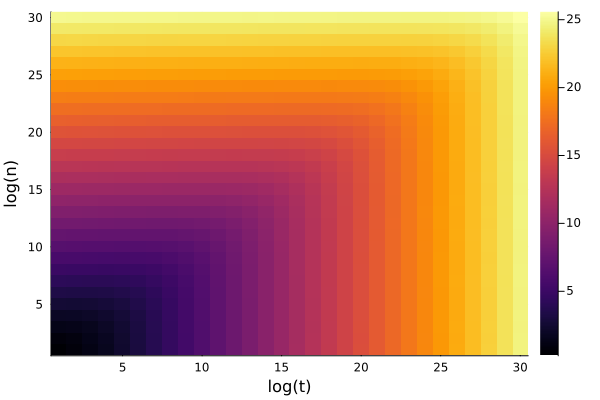
\includegraphics[width=\textwidth]{wykres.png}    
\end{center}


W przeciwieństwie do większości pozostałego kodu, który przygotowałem, ze względu na jednoczesne łatwe wykonywanie wykresów, oraz szybkość działania, 
eksperymentalne weryfikowanie, omawianej
hipotezy przeprowadziłem w języku Julia. Kod użyty do testowania znajduje się  w pliku \texttt{PrimesExperiment.jl}.

Omówię teraz już samą implementację modułu szukającego liczby pierwszej. Wszystkie wymienione niżej funkcje zostały  zaimplementowane w języku C++ i znajdują się w pliku \texttt{FindPrimes.cpp}.

Moduł losujący składa się z kilku funkcji, z których zdecydowanie najprostszą jest \texttt{pow2}, która dla przyjmowanej jako argument liczby \texttt{t}
zwraca najmniejszą potęgę \texttt{2} z wykładnikiem naturalnym, która jest większa niż \texttt{2t}. Polega ona na
mnożeniu przez \texttt{2} zmiennej \texttt{ans}, której początkowa wartość jest równa \texttt{1} dopóki nie będzie 
większa niż \texttt{2*t}. Musimy wykonać co najwyżej \texttt{126} mnożeń, co jest na tyle szybkie, że nie ma 
potrzeby stosowania bardziej zaawansowanych algorytmów jak na przykład 
używających algorytmu szybkiego potęgowania.


Funkcja \texttt{random128} służy do losowania dodatniej liczby typu
\texttt{\textunderscore \textunderscore int128} z przedziału $[0,1,...,m]$, gdzie $m$ to wartość zmiennej \texttt{mod}
typu \texttt{\textunderscore \textunderscore int128} podanej jako argument. 
Polega na losowaniu kolejnych bajtów zmiennej \texttt{ans} typu \texttt{\textunderscore \textunderscore int128}, a następnie,
zwróceniu wartości bezwzględnej jej reszty z dzielenia przez \texttt{mod}.

Sprawdzenie czy wylosowana liczba jest pierwsza wykonuję przy pomocy testu Millera-Rabina. 

Jego idea jest następująca: każdą liczbę pierwszą $p$ większą niż $2$ da się jednoznacznie zapisać w 
postaci $d2^s+1$
gdzie $d$ jest nieparzyste, zaś $s$ naturalne. Dla dowolnej liczby
$a \in \{2,3,...,p-1\}$ z małego twierdzenia Fermata $p$ dzieli

$$ a^{p-1}-1=a^{d2^s}-1=(a^d)^{2^s}-1=((a^d)^{2^{s-1}}+1)((a^d)^{2^{s-1}}-1)=$$


$$((a^d)^{2^0}-1)((a^d)^{2^0}+1)((a^d)^{2^1}+1)((a^d)^{2^2}+1)...((a^d)^{2^{s-1}}+1) $$

Tak więc z wyboru $a$ wiemy, że któraś z liczb  $(a^d)^{2^0}+1$, $(a^d)^{2^1}+1$,..., $(a^d)^{2^{s-1}}+1$
jest podzielna przez $p$, czyli dla pewnego $i \in \{0,1,2,...,s-1\}$ zachodzi, 

$$(a^d)^{2 ^i} + 1\equiv 0 \pmod p$$
czyli równoważnie 
$$(a^d)^{2 ^i} \equiv n-1\pmod p$$

Test Millera-Rabina opiera się na następującej obserwacji:
\begin{tcolorbox}
\textbf{Obserwacja 1:} Dla większej niż $2$ liczby $n=2^sd+1$, gdzie $s$ jest naturalne, zaś $d$ naturalne nieparzyste i liczby $
a \in \{2,3,...,n-1\}$,
jeżeli istnieje liczba $i \in \{0,1,2,..,s-1\}$ taka, że $(a^d)^{2^i} \equiv n-1 \pmod p$, to $n$
prawdopodobnie jest pierwsza. Jeżeli takie $i$ nie istnieje $n$ liczbą pierwszą na pewno nie jest.
\end{tcolorbox}

Prawdopodobieństwo błędu można minimalizować wybierając kilka liczb $a$. 
\begin{tcolorbox}
    \textbf{Fakt 1:} Jeżeli hipoteza Riemanna jest 
    prawdziwa wystarczające jest sprawdzenie $a$ z mniejszych lub równych
    $\min(n-2,2\ln^2(n))$ ~\cite{durnoga2017large}.
    
\end{tcolorbox}

Moja implementacja testu Millera Rabina składa z dwóch funkcji. 

Pierwsza z nich to \texttt{MillerRabinOne} mająca za zadanie sprawdzić warunek z \textbf{Obserwacji 1} dla określonych
\texttt{n} i \texttt{a} zwracając \texttt{false} gdy wiemy, że liczba nie jest pierwsza.
Na początku rozważam przypadki gdy \texttt{n} i \texttt{a} nie spełniają początkowych założeń dla, których
\textbf{Hipoteza 1} była formułowana przy pomocy następujących zapytań warunkowych:
\begin{lstlisting}
    if(n == 2) return true;
    if(n < 2) return false;
    if(n % 2==0) return false;
    if(a % n == 1) return true;
    if(a > n) return true;
\end{lstlisting}

Jeżeli warunki początkowe są spełnione, przy pomocy funkcji \texttt{field::setPsilly} ustawiam wartości pól statycznych klasy 
\texttt{field} tak, żeby symulowała
ona obliczenia w pierścieniu $\mathbb{Z}_n$. Oczywiście nie wszystkie działania zdefiniowane
w klasie \texttt{field} działają w pierścieniu $\mathbb{Z}_n$ (na przykład dzielenie). Jednak
możemy to zignorować po prostu ograniczając się do działań dodawania, odejmowania, mnożenia i potęgowania
z wykładnikiem naturalnym.

Wyznaczam \texttt{d} i \texttt{s} zgodnie z oznaczeniami z \textbf{Hipotezy 1}.

Następnie tworzę obiekt \texttt{x} klasy \texttt{field} z wartością pola \texttt{value} równą \texttt{a}.
Podnoszę \texttt{x} do potęgi \texttt{d} przy pomocy operatora \verb!^!\texttt{=} zdefiniowanego w module definiującym klasę \texttt{field}.
Następnie \texttt{s}-krotnie podnoszę w miejscu \texttt{x} do kwadratu przed każdym kolejnym podniesieniem sprawdzając, czy \texttt{x==n-1} 
co oznaczałoby, że liczba \texttt{n} jest ,,raczej pierwsza'' i zwracamy wtedy \texttt{true} lub \texttt{x==1} co oznaczałoby, że \texttt{x} po kolejnych podniesieniach do kwadratu
będzie wciąż równe \texttt{1}, więc \texttt{n} nie jest pierwsza i zwracamy \texttt{false}. Jeżeli żaden z tych warunków nigdy nie zaszedł 
po \texttt{s} podniesieniach do kwadratu zwracamy \texttt{false}.

Kolejną funkcją jest \texttt{MillerRabin}, która przyjmuje liczbę \texttt{n} typu \texttt{\texttt{\textunderscore \textunderscore int128}} i 
wywołuje funkcję \texttt{MillerRabinOne} z \texttt{n} jako pierwszym argumentem oraz drugim będącym kolejnymi liczbami ze zbioru
$\{2,3,...,\min(n-2, 2\ln^2(n))\}$ i jeżeli, któreś z tych wywołań zwróci \texttt{false} funkcja \texttt{MillerRabin} również 
zwraca \texttt{false}. Jeżeli jednak tak nie będzie to na podstawie \textbf{Faktu 1} zwracamy \texttt{true} oznaczające, że 
\texttt{n} z bardzo małym prawdopodobieństwem błędu jest pierwsza. 

Kolejną już ostatnią funkcją w tym module jest funkcja \texttt{find\_prime}. Przyjmuje ona jako argumenty liczbę \texttt{n} i 
\texttt{t}, zaś następnie, zwraca liczbę pierwszą postaci $r2^k+1$, gdzie $r$ jest liczbą naturalną z przedziału $[t+1,(n+t)^3]$.
Najpierw przy pomocy wywołania \texttt{srand((unsigned int)time(NULL))} wprowadzam losowość testu. 
Następnie przy pomocy funkcji \texttt{pow2} wyznaczam $2^k$. Następnie losuję potencjalne liczby \texttt{candidate} przy pomocy wywołania
funkcji \texttt{random128} na $(n+t)^3$. Jeżeli wylosuję liczbę nie większą niż \texttt{t} losuję jeszcze raz. Dla dużych \texttt{n} i \texttt{t}
prawdopodobieństwo tego jest znikome, a ewentualny koszt niewielki. Następnie mnożę
wylosowane $r$ z wyznaczonym $2^k$ i dodaję do wyniku $1$. Wynik tych operacji zapisuję w zmiennej \texttt{mod}.
Kolejnym krokiem jest dla tak uzyskanej liczby sprawdzenie, czy 
jest pierwsza przy pomocy funkcji \texttt{MillerRabin}. Jeżeli \texttt{m} i \texttt{t} są małe  może nie istnieć liczba pierwsza szukanej przez nas postaci, 
dlatego po wykonaniu \texttt{1000000} losowań ziększam \texttt{mod} dwukrotnie.



Omówione w tej sekcji funkcje znajdują się w pliku \texttt{find\_prime.cpp} i są napisane w języku C++.



\section{Teorioliczbowa szybka transformata Fouriera}

Dyskretna transformata Fouriera ~\cite{wang1984fast} służy przyspieszeniu mnożenia wielomianów. 
Wielomiany możemy reprezentować jako ciąg współczynników lub jako ciąg wartości w ustalonych punktach, 
których liczba przekracza stopień reprezentowanego wielomianu. Pierwsza reprezentacja jest wygodna
do wyliczania wartości w dowolnym punkcie z dziedziny, jednak mnożenie wielomianów w takiej postaci
jest czasochłonne i ma czas kwadratowy od długości wielomianów. Druga reprezentacja pozwala na 
mnożenie wielomianów w czasie liniowym, jednak wyliczanie ich wartości w innych punktach jest
trudne. Dyskretna transformata Fouriera służy do przechodzenia między tymi postaciami w 
relatywnie szybkim czasie $O(\log(n)n)$, gdzie $n$ to stopień tych wielomianów.

Wybór punktów opiera się na prostej obserwacji, że jeżeli $A(x) = a_0x^0+a_1x^1+..+a_{2n-1}x^{2n-1}$
(jeżeli stopień $A$ ma stopień parzysty przyjmujemy po prostu, że $a_{2n-1}$ jest równe $0$) jest równe
sumie $A_0(x^2)$, gdzie $A_0(t)=\sum_{i=0}^{n-1}a_{2i}t^{i}$, oraz 
$A_1(x^2)x$, gdzie $A_1(t)=\sum_{i=0}^{n-1}a_{2n+1}t^{i}$. Tak więc jeżeli dwie
liczby $a$ i $b$ mają te same wartości swoich kwadratów możemy obliczyć tylko raz wartości $A_1(a^2)=A_1(a^2)$ i $A_0(a^2)=A_0(b^2)$, 
a następnie, w czasie stałym połączyć te wyniki, tak aby uzyskać wartości 
wielomianu $A$ w punktach $a$ i $b$. 


Klasyczna wersja dyskretnej transformaty Fouriera oblicza wartości wielomianu $A$ dla
argumentów z ciała liczb zespolonych. Przyjmujemy następujące oznaczenie $A(x)=\sum_{i=0}^{\infty}a_ix^i$,
przy czym istnieje $I$ takie, że $\forall i>I: a_i = 0$. I oznaczając dalej 
$A_0(x) = a_0x^0+a_2x^1+..+a_{2^m-2}x^{2^{m-1}-1} $
oraz $A_1(x) = a_1x^1+a_3x^1+..+a_{2^m-1}x^{2^{m-1}-1} $, przy czym $2^m$ jest najmniejszą
potęgą $2$ o wykładniku naturalnym, większym niż stopień wielomianu będącego wynikiem optymalizowanego 
przez nas mnożenia. 

Będę oznaczał $\omega_m$ jako $e^{\frac{i2\pi}{2^m}}$. 
Zaważmy, że :
\begin{equation*}
  \systeme{
  A(\omega_m^1) = A_0(\omega_m^2)+A_1(\omega_m^2)\omega_m^1 = A_0(\omega_{m-1}^1)+A_1(\omega_{m-1}^1)\omega_m^1,
  A(\omega_m^2) = A_0(\omega_m^4)+A_1(\omega_m^4)\omega_m^2 = A_0(\omega_{m-1}^2)+A_1(\omega_{m-1}^2)\omega_m^2,
  A(\omega_m^3) = A_0(\omega_m^6)+A_1(\omega_m^6)\omega_m^3 = A_0(\omega_{m-1}^3)+A_1(\omega_{m-1}^3)\omega_m^3,
  \cdot \cdot \cdot ,
  A(\omega_m^{2^m}) = A_0(\omega_m^{2^{m+1}})+A_1(\omega_m^{2^{m+1}})\omega_m^{2^m} = A_0(\omega_{m-1}^{2^m})+A_1(\omega_{m-1}^{2^m})\omega_m^{2^m}}
\end{equation*}

Tak więc gdy mamy wektory $V_0=\Bigl( A_0(\omega_{m-1}^0),A_0(\omega_{m-1}^1),...,A_0(\omega_{m-1}^{2^{m-1}-1})\Bigr)$ oraz                          

$V_1=\Bigl( A_1(\omega_{m-1}^0),A_1(\omega_{m-1}^1),...,A_1(\omega_{m-1}^{2^{m-1}-1})\Bigr)$ możemy
w czasie liniowym od ich długości wyliczyć wektor $V=\Bigl( A(\omega_{m}^0),A(\omega_{m}^1),...,A(\omega_{m}^{2^{m}-1})\Bigr)$, jednak wyliczenie wektorów 
$V_1$ i $V_2$ można znów rozbić na wyliczenie, najpierw $2$ wektorów długości $2^{m-2}$ i 
następnie, połączenie tych dwóch wektorów w czasie liniowym od ich długości. Możemy tak rozbijać kolejne wektory aż dojdziemy do wektorów długości
$1$, które przechowują wartości pewnych wielomianów $0$-stopnia będących po prostu jednym ze współczynników $A$.

Niech $T(n)$ będzie czasem policzenia wartości wielomianu $A$ w $n=2^m$ punktach przy pomocy dyskretnej transformaty Fouriera. 
Fouriera. Wiemy, że $T(n)=2T(\frac{n}{2})+O(n)$. Rozwiązaniem takiego równania jest $T(n)=O(n\log(n))$.
Okazuje się, że po wyliczeniu wartości wielomianu $AB$ w omawianych punktach możemy ,,wyciągnąć'' z tych wartości w czasie
$O(n\log(n))$ wartości współczynników wielomianu $AB$, gdzie $n$ to ilość tych punktów, tak więc cały algorytm mnożenia odbywa się w czasie $O(\log(n)n)$.

Moja implementacja korzysta z dwóch klasycznych ulepszeń dyskretnej transformaty Fouriera. 

Pierwsza to tak zwana ,,Teorioliczbowa transformata Fouriera'' ~\cite{garg2017digital}. Polega ona na nie wykonywaniu obliczeń w ciele $\mathbb{C}$ lecz
w $\mathbb{Z}_p$, przy czym oczywiście musi w ciele tym istnieć pierwiastek z $1$ stopnia $2^m$, gdzie $2^m$ jest potęgą $2$ o wykładniku
naturalnym i większym niż stopień zwracanego wielomianu. 
Tak naprawdę oznacza to po prostu, że $p$ ma postać $r2^m+1$, gdzie $r$ jest liczbą naturalną, o czym pisałem w poprzedniej 
sekcji.

Jako $A[i:j]$ będę oznaczał komórki tablicy ze współczynnikami wielomianu $A$ o indeksach większych lub równych niż $i$ oraz mniejszych lub równych $j$. 


Drugim ulepszeniem jest użycie iteracyjnej szybkiej transformaty Fouriera ~\cite{wyrowski1988iterative}. Opiera się ona na obserwacji, że rekurencyjna wersja dyskretnej transformaty Fouriera 
polega, najpierw na podzieleniu współczynników wielomianu na coraz mniejsze grupy, aż do zawierających tylko pojedynczy współczynnik, a następnie, łączeniu pojedynczych współczynników
w pary zawierające informację o $2$ współczynnikach, potem czwórki, ósemki itd aż do połączenia ich w jeden duży blok zawierający informacje o wszystkich współczynnikach, a rekurencyjne wywołania służą jedynie 
pogrupowaniu w jakiej kolejności będziemy wykonywać łączenia.


Możemy jednak to grupowanie wykonać bez kolejnych rekurencyjnych wywoływań transformaty po prostu ustawiając obok siebie współczynniki w takiej kolejności 
żeby współczynniki wielomianów stopnia $2^l-1$, które w wersji rekurencyjnej powstają na $m-l$ poziomie rekursji
były w spójnych segmentach $A[0:2^l-1]$,$A[2^l:2 \cdot 2^l-1]$,
$A[2 \cdot 2^l:3\cdot 2^l-1]$,...,$A[(2^{m-l}-1)\cdot 2^l:2^m-1]$. Przy czym współczynniki wielomianu powstałego na
$l+1$ poziomie rekursji, które w wielomianie powstałym na $l$-tym poziomie rekursji były przy 
potęgach o wykładniku parzystym zostają umieszczone w ,,pierwszej połowie'' segmentu 
długości $2^l$, w którym były umieszczone na poprzednim etapie, zaś te, które były przy 
potęgach nieparzystych w drugim.

Zaważmy, że pierwsze ,,rozbicie'' wektora współczynników w wersji rekurencyjnej sprowadza się
do wybrania osobno współczynników parzystych i nieparzystych. Tak więc nasze grupowanie
powinno w polach o indeksach $(0,1,2,...,2^{m-1}-1)$ umieścić liczby znajdujące się, najpierw 
w polach o indeksach parzystych, czyli mające ostatni bit równy \texttt{0}, z kolei 
w polach o indeksach $(2^{m-1},2^{m-1}+1,...,2^m-1)$ powinno umieścić liczby nieparzyste, czyli
mające ostatni bit równy \texttt{1}. 

Pierwszy poziom rekursji rozbija wielomian
$A(x)=\sum_{i=0}^{2^m-1}a_ix^i$, na $A_0(x)=\sum_{i=0}^{2^{m-1}-1}a_{2i}x^{i}$ oraz
$A_1(x)=\sum_{i=0}^{2^{m-1}-1}a_{2i+1}x^{i}$. 

Gdy umieścimy współczynniki $A_0$ w $A[0:2^{m-1}-1]$, zaś $A_1$ w $A[2^{m-1}:2^m-1]$ należy umieścić 
współczynniki przy potęgach parzystych w wielomianie $A_0$ w pierwszej połówce 
$A[0:2^{m-1}-1]$, nieparzyste zaś w drugiej. I analogicznie współczynniki przy potęgach 
parzystych w wielomianie $A_1$ w pierwszej połówce 
$A[2^{m-1}:2^{m}-1]$, nieparzyste zaś w drugiej. To który współczynnik jest przy potędze 
parzystej czy nie w wielomianach $A_0$ i $A_1$ decyduje to czy początkowo był przy potędze,
której wykładnik miał drugi bit równy $0$, czy $1$. Dalsze kontynuowanie tego rozumowania 
prowadzi do wniosku, że jeżeli odwrócimy $m-1$ ostatnich bitów liczby $i$ otrzymamy numer komórki,
w której powinniśmy umieścić liczbę $a_i$. Istotnie załóżmy, że liczba powstała po odwróceniu $m$ ostatnich bitów liczby $i$ jest większa 
niż, że liczba powstała po odwróceniu $m$ ostatnich bitów liczby $j$. Prosta indukcja pozwala stwierdzić, że współczynniki, których indeksy mają $k$ 
wspólnych ostatnich 
bitów zostają na $k$-tym poziomie rekursji umieszczone w tym samym wielomianie. 
To czy zostaną umieszczone w pierwszej czy drugiej połowie segmentu, do którego były przypisane 
na $k$-tym poziomie rekursji zależy od tego czy ich $k+1$ bit jest równy $0$ czy $1$.

To, że liczba powstała po odwróceniu $m$ ostatnich bitów liczby $i$ jest większa niż liczba powstała po odwróceniu 
$m$ ostatnich bitów liczby $j$ oznacza, że pewna liczba $k$ (być może równa 
$0$) ostatnich bitów liczby $i$ jest taka sama jak liczby $j$ 
zaś $k+1$ ostatni bit liczby $i$ jest równy $1$, podczas gdy $k+1$ ostatni bit liczby $j$
jest równy $0$.
Tak więc do $k$-tego poziomu rekursji $a_i$ i $a_j$ pozostają w tym samym wielomianie $B(x)=
\sum^{2^{m-k}-1}_{l=0} b_lx^l$, czyli w wersji iteracyjnej są w tym samym segmencie 
długości $2^{m-k}$ i na $k+1$ poziomie rekursji w wersji rekurencyjnej $a_j$ jest umieszczane w wielomianie
ze współczynnikami $b_0,b_2,...,b_{2^{m-k}-2}$, zaś $a_i$ w wielomianie ze współczynnikami
$b_1,b_3,...,b_{2^{m-k}-1}$, tak więc w wersji iteracyjnej $a_j$ zostaje w umieszczone w pierwszej połowie 
segmentu, w którym są współczynniki $b_0$, $b_1$,..., $b_{2^{m-k}-1}$ zaś $a_i$ w drugiej, tak więc $a_i$ zostaje umieszczone w komórce o większym indeksie 
niż $a_j$. Ponieważ indeksy tablicy $A[0:2^m-1]$ 
wyznaczają wszystkie możliwe binarne liczby $m$-bitowe to istotnie, jeżeli odwrócimy $m-1$ ostatnich bitów liczby $i$ otrzymamy numer komórki,
w której powinniśmy umieścić liczbę $a_i$.


Przejdźmy do dokładnego opisu naszej implementacji. 

Najpierw definiuję funkcję \texttt{enoughGoodRoot}, która przyjmuje liczbę \texttt{k} typu 
\texttt{\textunderscore \textunderscore int128}
 i zwraca element typu \texttt{field}, który jest pierwiastkiem z \texttt{1} stopnia $2^k$. 
Jest to po prostu podniesienie elementu \texttt{field::almostPrimitiveRoot} (będącego pierwiastkiem z $1$ stopnia $2^{r}$, gdzie $r$
to wartość zmiennej \texttt{field::degreeOfDegree}) \texttt{field::almostPrimitiveRoot-k}
razy do kwadratu.





Kolejnym etapem jest odpowiednie ustawienie wartości w komórkach wektora ze współczynnikami wielomianu 
(nazwę go \texttt{coefficients}) tak by można było wykonać na nim iteracyjną wersję szybkiej transformaty Fouriera. 



Funkcja \texttt{reverseBits} służy znalezienia indeksu komórki, w której powinna być umieszczona 
liczba znajdująca się początkowo w komórce o indeksie \texttt{x}, gdzie \texttt{x} jest pierwszym 
argumentem funkcji \texttt{reverseBits} typu
\texttt{long long}, zaś drugim argumentem jest liczba \texttt{k} 
typu \texttt{long long} wyznaczająca ile ostatnich bitów \texttt{x} należy odwrócić.

Na początku zamieniamy miejscami bity o indeksach parzystych \texttt{x} z nieparzystymi.
Robimy to, najpierw tworząc dwie kopie zmiennej \texttt{x}. W jednej z nich zerujemy 
(and-ując ją z odpowiednią maską) bity o indeksach parzystych, zaś w drugiej nieparzystych.
Pierwszą kopię przesuwamy o $1$ bit w prawo, tak, że bity o indeksach parzystych stały się bitami
o indeksach nieparzystych, zaś drugą w lewo i wykonujemy na tak zmodyfikowanych kopiach operację
\texttt{or}-a bitowego. 

Analogiczną operację jak omówiona w poprzednim akapicie dla bloków składających się z $1$-bitowych 
wykonujemy na blokach $2$-bitowych, $4$-bitowych, $8$-bitowych, $16$-bitowych,
i $32$-bitowych. 

Tak zmodyfikowana zmienna \texttt{x} jest odwróconą bitowo początkową wartością zmiennej 
\texttt{x}. Ponieważ chcieliśmy odwrócić jedynie jej ostatnie \texttt{k} bitów przed 
zwróceniem \texttt{x} jako wyniku przesuwamy ją jeszcze o \texttt{64-k} bitów w prawo bez znaku.






Gdy mamy już funkcję \texttt{reverseBits} możemy stworzyć funkcję \texttt{setToDo} transformującą wektor współczynników w wektor gotowy
do wyliczenia jego szybkiej transformaty Fouriera. Jako argumenty dla tej funkcji otrzymujemy wektor elementów typu \texttt{field} o nazwie 
\texttt{coefficients} oraz 
zmienną \texttt{long long} o nazwie \texttt{size} oznaczającą żądaną długość wektora wynikowego (jest to odpowiednio duża potęga dwójki o wykładniku naturalnym). 
Na początku dopełniamy wektor 
\texttt{coefficients} elementami równymi \texttt{field(0)} do rozmiaru \texttt{size}. 
W zmiennej \texttt{log} zapisujemy wartość logarytmu o podstawie $2$ na argumencie będącym długością
wektora \texttt{coefficients}.
Następnie w pętli z iteratorem \texttt{i} przechodzącym po wszystkich liczbach naturalnych od \texttt{0} do 
\texttt{size-1} i jeżeli \texttt{reverseBits(i,log) > i} (warunek ten służy temu, by każdy element został zamieniony dokładnie raz. 
Zauważmy też, że \texttt{reverseBits(reverseBits(i,log),log)=i}) zamieniam w tabeli pole o indeksie \texttt{i} z polem o indeksie 
\texttt{reverseBits(i,log)} miejscami. Funkcja nic nie zwraca, a jedynie modyfikuje wektor podany jako argument.

Przejdźmy do funkcji \texttt{DFT}, która otrzymując wektor współczynników wielomianu \texttt{coefficients}, 
liczbę \texttt{size} nie mniejszą niż długość tego wektora i będący potęgą $2$ o wykładniku naturalnym oraz obiekt \texttt{omegaM} typu \texttt{field},
który jest pierwiastkiem z \texttt{1} stopnia \texttt{size} zwraca wektor zawierający wartości tego wielomianu w punktach kolejno 
\texttt{omegaM}\verb!^!\texttt{0}, \texttt{omegaM}\verb!^!\texttt{1},..., \texttt{omegaM}\verb!^!\texttt{size-1}. 

Poniżej umieściłem kod tej procedury.

\begin{lstlisting}
void inline DFT(std::vector<field>&coefficients, long long size, field omegaM){
    setToDo(coefficients,size);
    std::stack<field> omegasM;
    while(omegaM != 1){
        omegasM.push(omegaM);
        omegaM *= omegaM;
    }
    long long m = 1;
    while(!omegasM.empty()){   
        field currentOmegaM= omegasM.top();
        omegasM.pop();
        field omega = 1;
        m*=2;
        for(long long j = 0; j<m/2;j+=1){
            for(long long k = j; k<size; k+=m){
                field t = omega * coefficients[k+m/2];
                field u = coefficients[k];
                coefficients[k] = u+t;
                coefficients[k+m/2] =  u - t;
            }
            omega *= currentOmegaM;
        }
    }
}
\end{lstlisting}



Na początku przygotowujemy wektor do wykonania dalszej części obliczeń wywołując zdefiniowaną wcześniej funkcję \texttt{setToDo} na wektorze 
\texttt{coefficients} i dla liczby \texttt{size}. 

Tworzymy stos, na który kładziemy wyniki kolejnych złożeń podniesienia do kwadratu liczby \texttt{omegaM} aż do \texttt{-1}.

Póki stos nie będzie pusty, będę w każdej iteracji pętli \texttt{while} ściągał z niego kolejne wartości i przypisywał je do zmiennej \texttt{currentOmegaM}.

W dalszej części będę oznaczał jako $\omega_i$ pierwiastek z $1$ stopnia $2^i$, w $\mathbb{Z}_p$.

Przyjmijmy oznaczenie, że na początku \texttt{i}-tej iteracji wektor \texttt{coefficients} ma postać $\frac{size}{2^{i-1}}$ bloków postaci
$(f_{i,k}(\omega_i^0), f_{i,k}(\omega_i^1), ...,f_{i,k}(\omega^{2^{i-1}-1}_i))$, gdzie $k$ to numer bloku. Chcemy
następujące po sobie pary bloków połączyć w jeden blok postaci $(f_{i+1,k}(\omega_{i+1}^0),f_{i+1,k}(\omega_{i+1}^1),...,
f_{i+1,k}(\omega^{2^{i}-1}_{i+1}))$, przy czym 
$f_{i+1,k}(\omega_{i+1}^j) = f_{i,2k}(\omega_{i}^\frac{j}{2})+f_{i,2k+1}(\omega_{i}^{\frac{j}{2}})\omega_{i+1}^j$. 

Kolejne iteracje pętli z iteratorem \texttt{j} odpowiadają kolejnym punktom, w których obliczamy wartości odpowiednich wielomianów, zaś pętli z iteratorem 
\texttt{k}
numerom kolejnych rozpatrywanych wielomianów. Ponieważ $\omega_{i+1}^{2^i}=-1$ wyliczenie $f_{i+1,k}(\omega_{i+1}^{j})$ i $f_{i+1,k}(\omega_{i+1}^{j+2^i})$ 
wyliczam w jednej iteracji pętli.


Przejdźmy do pełnej procedury mnożenia. 
\begin{lstlisting}
std::vector<field>multiplication(std::vector<field> A, std::vector<field> B){
    long long size = 1;
    while(size < (long long)((A.size() + B.size()) +2 )){
        size *= 2;
    }
    long long l = log(size);
    field omegaM = enoughGoodRoot(l);
    DFT(A,size,omegaM);  
    DFT(B,size,omegaM);
    for(long long i=0;i<size;i++){
        A[i] = B[i] * A[i]; 
    }
    omegaM = field(1)/omegaM;
    DFT(A,size,omegaM);
    for(long long i=0;i<size;i++){
        A[i] /= field(size);
    } 
    return A;
}
\end{lstlisting}
Wektorów nie przekazuję przez referencje bo je modyfikuję.

Najpierw wliczamy wartość \texttt{size} będącą liczbą punktów, w których będziemy liczyć wartości wielomianu $AB$ (jest to najmniejsza liczba będąca potęgą 
$2$ o wykładniku naturalnym większa niż stopień $AB$). Kolejnym etapem jest znalezienie pierwiastka stopnia \texttt{size} z \texttt{1} w $\mathbb{Z}_p$. 
Następnie wyliczamy przez wywołania \texttt{DFT} na odpowiednich argumentach wektor $(A(omegaM^0),A(omegaM^1),...,A(omegaM^{s-1}))$, 
oraz $(B(omegaM^0),B(omegaM^1),...,B(omegaM^{s-1}))$, gdzie $s$
to wartość zmiennej \texttt{size}. Następnie w kopii wektora \texttt{A} zapisuję wartości $AB$ w kolejnych punktach będące wartościami odpowiednich 
mnożeń.

Okazuje się, że aby zmienić, wektor $(AB(omegaM^0),AB(omegaM^1),...,AB(omegaM^{s-1}))$, gdzie $s$ jest wartością zmiennej \texttt{size}
w wektor kolejnych współczynników $AB$ wystarczy wywołać na nim \texttt{DFT} z drugim argumentem równym \texttt{size} i trzecim 
będącym równym odwrotności \texttt{omegaM} w $\mathbb{Z}_p$, a następnie, podzielić w $\mathbb{Z}_p$ każdy jego element przez $size$. 























\section{Pochodna algebraiczna i jej własności}
Klasyczna analityczna definicja pochodnej jest to przekształcenie funkcji $f(x)$ w funkcję $f'(x)$ taką, że
$f'(x)=\lim_{h \to 0}\frac{f(x+h)-f(x)}{h}$. Definicja taka traci jednak cały sens jeżeli chcemy zmienić dziedzinę
funkcji $f$ i $f'$ z liczb rzeczywistych na dziedzinę, gdzie nie możemy zmniejszać $h$ w taki sposób, by było 
dowolnie małe lecz niezerowe. Przykładem takiej dziedziny jest ciało $\mathbb{Z}_p$. 

Zauważmy, że jeżeli funkcja $f$ $\mathbb{R}\to \mathbb{R}$ jest gładka w okolicy $0$, możemy ją utożsamić z jej szeregiem Taylora $\sum_{i=0}^{\infty}f_ix^i$. 

Weźmy liczbę pierwszą $p$. W dalszej części sekcji będę zakładał, że współczynniki szeregu Taylora 
rozważanej funkcji są postaci 
$\frac{a_i}{b_i}$, gdzie $a,b \in \mathbb{Z}$ i  $b$ jest niepodzielne przez $p$. Przy takim założeniu napis  
$\sum_{i=0}^{\infty}\frac{a_i}{b_i}x^i$ zachowuje algebraiczny sens również w ciele reszt $\mathbb{Z}_p$, w którym 
liczbę całkowitą utożsamiamy z jej resztą z dzielenia przez $p$. W języku szeregów Taylora pochodną można 
zdefiniować jako przekształcenie funkcji $f(x)=\sum_{i=0}^\infty f_ix^i$ w funkcję 
$f '(x)=\sum_{i=0}^{\infty}(i+1)f_{i+1}x^i$. 

Udowodnię teraz, że tak zdefiniowana pochodna, dla funkcji $f(x)=\sum_{i=0}^{\infty}f_ix^i$ i
$g(x)=\sum_{i=0}^{\infty}g_ix^i$ zachowuje własności $f'+g'=(f+g)'$, $f'-g'=(f-g)'$, $(fg)'=f'g+fg'$ oraz 
$f(g)'=f'(g)g'$.

\begin{tcolorbox}
    \textbf{Lemat:} $f'+g'=(f+g)'$ oraz $f'-g'=(f-g)'$
    
    \textbf{Dowód:} $f'+g'=\sum_{1}^{\infty}if_ix^{i-1}+\sum_{1}^{\infty}ig_ix^{i-1}=
    \sum_{1}^{\infty}i(f_i+g_i)x^{i-1}=(f+g)'$ i analogicznie
    
    $f'-g'=\sum_{1}^{\infty}if_ix^{i-1}-\sum_{1}^{\infty}ig_ix^{i-1}=
    \sum_{1}^{\infty}(f_i-g_i)x^{i-1}=(f-g)'$ 
\end{tcolorbox}

\begin{tcolorbox}
    \textbf{Lemat:} $(fg)'=f'g+fg'$.
    
    \textbf{Dowód:} $(fg)'=((\sum_{i=0}^{\infty}f_ix^i)(\sum_{i=0}^{\infty}g_ix^i))'=
    (\sum_{i=0}^{\infty}(\sum_{j=0}^if_jg_{i-j})x^i)'=
    \sum_{i=1}^{\infty}(\sum_{j=0}^if_jg_{i-j})ix^{i-1}=
    \sum_{i=0}^{\infty}(\sum_{j=0}^if_jg_{i+1-j})(i+1)x^{i}$ z kolei

    $f'g+fg'=(\sum_{0}^{\infty}(i+1)f_{i+1}x^{i})(\sum_{i=0}^{\infty}g_ix^i)+(\sum_{0}^{\infty}(i+1)g_{i+1}x^{i})(\sum_{i=0}^{\infty}f_ix^i)=
    \sum_{i=0}^\infty(\sum_{j=0}^{i}f_{i+1-j}g_{j}(i+1-j))x^i+
    \sum_{i=0}^\infty(\sum_{j=0}^{i}g_{i+1-j}f_{j}(i+1-j))x^i=
    \sum_{i=0}^\infty(\sum_{j=0}^{i}g_{i+1-j}f_{j}(i+1-j+j))x^i=
    \sum_{i=0}^\infty(\sum_{j=0}^{i}g_{i+1-j}f_{j})(i+1)x^i=(fg)'
    $
\end{tcolorbox}

\begin{tcolorbox}
    \textbf{Lemat:} $(f(g))'=f'(g)g'$.
    
    \textbf{Dowód:} Na początek przyjmijmy, że $f(x)=x^k$, gdzie $k$ jest liczbą naturalną. Dla $k=0$ i $k=1$ teza jest 
    spełniona. Niech teza jest spełniona dla $f(x)=x^l$ oraz dla każdego naturalnego $k$ mniejszego niż $l$.
    Wtedy
    $(g^k)'=((g^{k-1})g)'=(g^{k-1})g'+g(g^{k-1})'=(g^{k-1})g'+g((k-1)g^{k-2}g')=
    (g^{k-1})g'+((k-1)g^{k-1}g')=kg^{k-1}g'$, tak więc na mocy zasady indukcji dla dowolnego $k$ naturalnego jeżeli $f(x)=x^k$ to $(f(g))'=f'(g)g'$ dla dowolnego $g$ postaci $\sum_{0}^{\infty}g_ix^i$. W takim razie dla dowolnego $f$
    postaci $\sum_{0}^{\infty}f_ix^i$ zachodzi,  $(f(g))'=(\sum_{i=0}^{\infty}f_ig(x)^i)'=\sum_{i=0}^{\infty}f_i(g(x)^i)'=
    \sum_{i=0}^{\infty}f_i ig^{i-1}(x)g'=f'(g)g'$.

    
    
    
    
    
    
    
    %$f'(g)g'=(\sum_{i=0}^{\infty}f_{i+1}(i+1)g(x)^i)(\sum_{i=0}^{\infty}(i+1)g_{i+1}x^i)$
    
\end{tcolorbox}


\section{Implementacja algorytmu Jin i Wu}
W tej części pracy dla funkcji $F(x)$, której szereg Taylora ma postać $\sum_{i=0}^{\infty}f_ix^i$ jako $F_t$ będziemy
oznaczać $\sum_{i=0}^{t}f_ix^i$.

Zasadnicza implementacja algorytmu Jin i Wu składa się z $4$ funkcji. 

Pierwszą z nich jaką omówię jest funkcja \texttt{B}, której zadaniem jest wyliczenie pierwszych 
$t+1$ współczynników szeregu Taylora $B(x)=\ln(\prod_{i=1}^n(1+x^{s_i}))$.

Funkcja \texttt{B} wyznacza wektor $t+1$ pierwszych wyrazów szeregu Taylora w ciele $\mathbb{Z}_p$ następującej 
funkcji:
$$
B(x)=\ln\prod_{i=1}^n((1+x^{s_i}))=\sum_{i=1}^n \ln(1+x^{s_i})=\sum_{i=1}^n(\sum_{j=1}^\infty
\frac{(-1)^{j-1}}{j}x^{s_i j})
$$

Niech $a_k$ będzie oznaczać liczbę elementów $S$ równych $k$.

Przy tak przyjętych oznaczeniach 

$$
B_t(x)=\sum_{i=1}^n (\sum_{j=1}^{\lfloor \frac{t}{s_i} \rfloor}\frac{(-1)^{j-1}}{j}x^{s_ij})
=\sum_{k=1}^t (\sum_{j=1}^{\lfloor \frac{t}{k} \rfloor}\frac{a_k(-1)^{j-1}}{j}x^{jk})$$

Spójrzmy na implementację funkcji \texttt{B}.

\begin{lstlisting}
std::vector<field> B(std::vector<field> s, long long t){
    std::vector<field> a(t+1,field(0));
    std::vector<field> ans(t+1,field(0));
    int K;
    for(int i =0; i<s.size(); i++){
        if(s[i].getValue()<=t)a[s[i].getValue()] ++;
    }
    for(long long k = 1; k <= t; k++){
        for(long long j = 1; j <= t/k ; j++){
            field x = field(-1);
            ans[k*j] = ans[k*j] + a[k]*(x^(j-1))/field(j);
        }
    }
    return ans;
}
\end{lstlisting}

Na początku tworzę wektor \texttt{a}, którego \texttt{k}-ty element oznacza zdefiniowane wcześniej $a_k$. 
Reszta kodu jest prostym przetłumaczeniem matematycznej notacji sumy na składnię zawierającą pętle, przy 
czym pole \texttt{ans[i]} odpowiada współczynnikowi przy $x^i$ w rozwinięciu w szereg Taylora funkcji $B(x)$.

Kolejne dwie funkcje to \texttt{compute} i \texttt{mainCompute}. 



Ich celem jest wyliczenie współczynników $(\exp(B(x)))_t=(\sum_{i=0}^\infty \frac{B(x)^i}{i!})_t$

Algorytm ten bazuje na spostrzeżeniu, że żeby wyliczyć $G_t(x)$, gdzie $G(x)=\exp(F(x))$ i $F(x) =\sum_{i=1}^\infty f_ix^i$,
jeżeli znamy $G(0)$ wystarczy znaleźć wartości $f_0,f_1,...,f_t$. Co więcej $G_t(F(x))=G_t(F_t(x))$

Niech rozwinięcie w szereg Taylora funkcji $G$ ma postać $\sum^{\infty}_{i=0}g_ix^i$

Zauważmy, że $G'(x)=(\exp(F(x)))'=\exp(F(x))F'(x)=G(x)F'(x)$, tak więc
$\sum_{i=0}^{\infty}(i+1)g_{i+1}x^{i}=(\sum_{i=0}^{\infty}g_ix^i)(\sum_{i=1}^{\infty}if_{i}x^{i-1})=
\sum_{i=0}^{\infty}(\sum_{j=1}^{i+1}jf_jg_{i+1-j})x^i$

Tak więc $(i+1)g_{i+1}=\sum_{j=1}^{i+1}jf_jg_{i+1-j}$, czyli $g_{i+1}=(i+1)^{-1}(\sum_{j=1}^{i+1}jf_jg_{i+1-j})$.
Zauważmy, że $G(0)=g_0$, tak więc mając wyliczone $f_0,f_1,...,f_t$ jesteśmy w stanie po kolei wyliczyć $g_1,g_2,...,g_t$.

Weźmy liczbę pierwszą $p>t$.

$B(x)=\ln(\prod_{i=0}^n(1+x^{s_i}))=\sum_{i=1}^{n}(\sum_{k=1}^{\infty}\frac{(-1)^{k-1}x^{s_ik}}{k}):=\sum_{i=0}^{\infty}b_ix^i$, 
więc każda z liczb $b_0,b_1,...,b_t$ da się zapisać jako liczba wymierna postaci $\frac{x}{y}$, gdzie $x,y$ to
względnie pierwsze liczby naturalne i $y$ nie jest podzielne przez $p$. Jeżeli $x$ i $y$ utożsamimy z resztą dzielenia ich 
przez $p$ to wartość wyrażenia $\frac{x}{y}$ da się wyliczyć w ciele $\mathbb{Z}_p$.

Niech $A(x)=\exp(B(x))=\prod_{i=0}^n(1+x^{s_i}):=\sum_{i=0}^{\infty}a_ix^i$.

Wiemy, że $a_{i+1}=(i+1)^{-1}(\sum_{j=1}^{i+1}jb_ja_{i+1-j})$, a także $a_0=\prod_{i=0}^n(1+0^{s_i})=1$, więc każda
z liczb $a_i$, gdzie $i \in \{0,1,2,..,t \}$ da się przedstawić w postaci $\frac{X_i}{Y_i}$, gdzie $X_i,Y_i$ to
względnie pierwsze liczby naturalne i $Y_i$ nie jest podzielne przez $p$. Jeżeli $X_i$ i $Y_i$ utożsamimy z resztą dzielenia ich 
przez $p$ to wartość wyrażenia $\frac{X_i}{Y_i}$ da się wyliczyć w ciele $Z_p$ i wartość liczby $a_i$ dla naturalnego $i$
nie większego niż $t$ jest równa $0$ wtedy i tylko wtedy gdy dla jej postaci $\frac{X_i}{Y_i}$ $p$ dzieli $X_i$. Zauważmy,
że $A(x)$ jest iloczynem wielomianów o całkowitych współczynnikach, więc też jest wielomianem o całkowitych współczynnikach,
więc $a_i$ jest wartością całkowitą, która w ciele $Z_p$ jest utożsamiona z $0$ wtedy i tylko wtedy, gdy jest podzielna przez $p$.

Na mocy powyższych rozważań, wykonuję dalsze obliczenia w ciele $\mathbb{Z}_p$, chyba, że explicite zaznaczę inaczej.


Procedura \texttt{mainCompute} jako argument przyjmuje wektor \texttt{f} $t+1$ pierwszych współczynników rozwinięcia w 
szereg Taylora funkcji $B$. Na początku inicjuje wynikowy $t+1$-elementowy wektor \texttt{g} ustawiając wszystkie
jego komórki poza \texttt{g[0]} na \texttt{0}, z kolei \texttt{g[0]} ustawiamy na \texttt{1}. Następnie uruchamiamy funkcję 
\texttt{compute} na argumentach \texttt{0}, \texttt{t}, \texttt{g} i \texttt{f}.

Funkcja \texttt{compute} zapisuje do wektora podanego jako trzeci argument (oczywiście przez referencję, żeby 
można było go modyfikować) wartości kolejnych współczynników szeregu Taylora funkcji 
$g(x)=\exp(\sum_{i=0}^tf_ix^i)$, gdzie $t+1$ to długość wektora podanego jako czwarty argument, zaś
$f_i$ to wartość \texttt{i}-tej komórki wektora podanego jako czwarty argument. W dalszej części jako $f_i$ będę 
oznaczał wartość \texttt{i}-tej komórki wektora podanego jako czwarty argument, zaś jako $g_i$ będę oznaczał wartość 
\texttt{i}-tej komórki wektora podanego jako trzeci argument. Nie będę traktować $g_i$ jak ,,zwykłą''
liczbę, ale wartość zmieniającą się w czasie wykonywania programu, gdy zmienia się wartość odpowiadającej jej
komórki wektora.
Jako $t$ będę oznaczał \texttt{f.size()-1}

Idea funkcji \texttt{compute} bazuje na tym, że aby wyliczyć $g_i=(i+1)^{-1}(\sum_{j=1}^{i+1}jf_jg_{i+1-j})$ dla wszystkich $i \in \{1,2,...,t\}$ należy
wykonać $O(n^2)$ dodawań składników postaci $(i+1)^{-1}jf_jg_{i+1-j}$ do odpowiednich komórek. Nie każde dodawanie można wykonać w dowolnym
momencie, ponieważ wartości komórek wektora \texttt{g} ulegają zmianie. Dodawanie uznamy za dozwolone, jeżeli $g_{i+1-j}$ obecne w 
dodawanym składniku $(i+1)^{-1}f_jg_{i+1-j}$ nie ulega zmianie. 

Zapisana w pseudokodzie funkcja \texttt{compute} ma postać:

\begin{verbatim}
procedure compute(l,r,g,f)
    if l < r
        m <- floor((l+r)/2) #obliczenia w tej linii wykonujemy w liczbach naturalnych
        compute(l,m,g,f)
        for i <- m+1, m+2,...,r
            for j<-l,l+1,..,m
                g[i] <- g[i]+(i-j)f[i-j]g[j]/i
            end for
        end for
        compute(m+1,r,g,f)
    end if
end procedure
\end{verbatim}

Po wykonaniu \texttt{compute(l,r,f,g)} chcemy, żeby wartości $g_l,g_{l+1},...,g_{r}$ były już ustawione na wartości docelowe, zaś
przed wykonaniem \texttt{compute(l,r,f,g)} chcemy, żeby wszystkie składniki postaci $(i+1)^{-1}f_jg_{i+1-j}$, gdzie $i+1-j<l$ zostały
już dodane do odpowiednich komórek \texttt{g} o indeksach należących do $\{0,1,...,r\}$. Chcemy też, żeby każda operacja dodawania
była dozwolona. 

Jeżeli długość \texttt{g} jest równa $0$ to żądania napisane w poprzednim akapicie są spełnione. 
Załóżmy indukcyjnie, że są spełnione dla \texttt{g} długości $0,1,2,..,t-1$. Niech długość \texttt{g} jest równa $t$.

Wywołanie \texttt{compute(0,t,f,g)} sprowadza się najpierw do wywołania rekurencyjnego \texttt{compute(0,m,f,g)}, gdzie \texttt{m} to wynik wykonanej w
liczbach całkowitych działania $\lfloor \frac{t}{2}\rfloor$. Po jej wykonaniu z tezy indukcyjnej $g_0,g_2,...,g_m$ mają docelowe
wartości. Następnie przechodzimy do wykonania pętli
\begin{verbatim}
for i <- m+1, m+2,...,r
    for j<-l,l+1,..,m
        g[i] <- g[i]+(i-j)f[i-j]g[j]/i
    end for
end for
\end{verbatim}

Ponieważ indeks \texttt{j} jest nie większy niż \texttt{m}, wszystkie dodawania są dozwolone. 
Po wykonaniu tej pętli zostają już wykonane wszystkie
potrzebne dodania wyrazów postaci \texttt{g[i]+(i-j)f[i-j]g[j]/i}, gdzie \texttt{j} jest nie większe niż \texttt{m}. 
Następnie wykonujemy \texttt{compute(m+1,r,g,f)}, co przypomina wywołanie \texttt{compute(0,r-m-1,f,g)} z tą modyfikacją, że w momencie 
gdy wykonalibyśmy linię \texttt{g[i] <- g[i]+(i-j)f[i-j]g[j]/i} każde wystąpienie
zmiennych \texttt{i} i \texttt{j} zastępujemy odpowiednio zmiennymi \texttt{i+m+1} i \texttt{j+m+1}. Ponieważ zgodnie z tezą
indukcyjną po wykonaniu \texttt{compute(0,r-m-1,f,g)},
$g_i$ zostaje zwiększone o $(i+1)^{-1}(\sum_{j=1}^{i+1}jf_jg_{i+1-j})$, dla $i \in \{1,2,...,r-m-1\}$ 
to po wykonaniu \texttt{compute(m+1,r,f,g)}, $g_{i+m+1}$  zostaje zwiększone o $(m+1+i+1)^{-1}(\sum_{j=1}^{i+1}jf_{m+1+j}g_{m+1+i+1-j})$, 
dla $i \in \{1,2,...,r-m-1\}$, więc po wykonaniu \texttt{compute(m+1,r,g,f)} $g_i=(i+1)^{-1}(\sum_{j=1}^{i+1}jf_jg_{i+1-j})$ dla każdego
$i \in \{0,1,2,3,...,t\}$. 

Nasza implementacja jednak korzysta z jednego usprawnienia. Zauważmy, że iloczyn wielomianów $F(x)=\sum_{k=0}^{r-l}kf_kx^k$ i 
$G(x)=\sum_{j=0}^{m-l}g_{j+l}x^j$, ma postać 
$\sum_{i=0}^{r+m-2l}(\sum_{k=0}^{r-l}kf_kg_{i-k+l})x^i$, tak więc w tym iloczynie współczynnik przy potędze $x^{i-l}$ podzielony
przez $i$ jest równy liczbie, o którą zostaje zwiększone $g_i$ po wykonaniu pętli
\begin{verbatim}
for i <- m+1, m+2,...,r
    for j<-l,l+1,..,m
        g[i] <- g[i]+(i-j)f[i-j]g[j]/i
    end for
end for
\end{verbatim}

Wykonanie pętli naiwnie zajmuje czas $O(t^2)$, zaś wykorzystanie szybkiej teorioliczbowej transformaty Fouriera do mnożenia wielomianów,
w mojej implementacji przyspieszyć wykonanie tej pętli do $O(t\ln(t))$.
Niech $T(t)$ oznacza czas wykonania \texttt{compute}, gdzie różnica między drugim i pierwszym argumentem wynosi $t+1$.
Ponieważ $T(t)=2T(\frac{t}{2})+O(t\ln(t))$, to $T(t)=O(t \ln^2(t))$.

Kolejną ostatnią już implementowaną przeze mnie funkcją jest \texttt{JinWu}. Przyjmuje ona wektor \texttt{s} 
elementów zbioru 
$S$, oraz
liczbę \texttt{t}. Najpierw losuje ona liczbę pierwszą \texttt{p}, która jest wynikiem wykonania funkcji 
\texttt{find\_prime(s.size(),t)}. Następnie
wywołując \texttt{field::setP(p)} ustawiam zmienne statyczne klasy \texttt{field} tak, żeby obliczenia w niej wykonywane 
odpowiadały wykonaniu ich w klasie $\mathbb{Z}_p$. Potem do wektora \texttt{Bans} przy pomocy wykonania funkcji 
\texttt{B(s,t)} zapisuję
$t+1$ pierwszych współczynników(w $\mathbb{Z}_p$) szeregu Taylora funkcji $B(x)=\ln(\prod_{i=0}^{n-1}(1+x^{s_i}))$, gdzie jako $n$ oznaczam długość
wektora \texttt{s}, zaś jako $s_i$ oznaczam jego $i$-tą komórkę w $\mathbb{Z}_p$ (będę to oznaczenie stosował również w dalszej części pracy). 
Następnie do wektora \texttt{computeAns} zapisuję $t+1$ pierwszych współczynników(w $\mathbb{Z}_p$) szeregu Taylora funkcji 
$A(x)=\prod_{i=0}^{n-1}(1+x^{s_i})$ jako wynik procedury \texttt{mainCompute(t,Bans)}. 
Zauważmy, że ponieważ $A(x)$ jest wielomianem współczynnik
przy potędze $x^i$ w jego rozwinięciu w szereg Taylora jest po prostu współczynnikiem przy potędze $x^i$ w wielomianie $A(x)$, zaś współczynnik przy potędze $x^i$ w $A(x)$ oznacza ilość sposobów wybrania ciągu indeksów naturalnych $-1<i_1<i_2<...<i_m<n$, 
takich, że
$x^{s_{i_1}+s_{i_2}+...+s_{i_m}}=x^i$, czyli liczba podzbiorów $S$ dających sumę $i$. Ponieważ liczby te zapisujemy jako elementy 
$\mathbb{Z}_p$ możliwe, \texttt{computeAns[t]} jest równe $0$ mimo, że istnieją podzbiory $S$ o sumie $t$ jednak ich liczba jest podzielna
przez $p$. Jednak liczba tych podzbiorów na pewno jest nie większa niż $2^n$, więc ma co najwyżej $n$ różnych czynników pierwszych.
Eksperymenty w sekcji poświęconej losowaniu liczby pierwszej pozwalają założyć, że liczba możliwych do wylosowania wartości $p$
jest $O(\frac{(n+t)^3}{\log(n+t)})=O((n+t)^2)$, więc prawdopodobieństwo, że $p$ dzieli niezerową liczbę podzbiorów $S$ o sumie $t$
jest $O(\frac{n}{(n+t)^2})=O(\frac{1}{n+t})$.

\section{Wyniki}
Poniżej prezentuję wyniki działania mojego algorytmu w porównaniu z algorytmem klasycznym omówionym w sekcji drugiej
używającym \texttt{bitset}-u o \texttt{10000000} elementów.
Testy zostały wykonane na komputerze z procesorem \texttt{Intel i5-7300HQ (4) @ 3.500GHz}. Niestety nawet dla dużych
danych nie udało się osiągnąć przewagi nad algorytmem dynamicznym.

\begin{verbatim}
n=100000 t=2000000
Jin Wu time =935s
Brutal time =530s
poprawne 2000001/2000001
_______________________________________________________
n=200000 t=3000000
Jin Wu time =1961s
Brutal time =580s
poprawne 3000001/3000001
_______________________________________________________
n=300000 t=4000000
Jin Wu time =2455s
Brutal time =1627s
poprawne 4000001/4000001
_______________________________________________________
n=400000 t=5000000
Jin Wu time =2576s
Brutal time =2062s
poprawne 5000001/5000001
_______________________________________________________
\end{verbatim}
    
\bibliographystyle{plain}
\bibliography{bibliography.bib}

\end{document}
